\documentclass[10pt,a4paper]{article}
\usepackage[margin=25mm]{geometry}
\usepackage{amsmath,amssymb,amsthm,mathtools,graphicx,hyperref,stmaryrd}
\sloppy
\setlength{\tabcolsep}{2pt}
\title{Transfinite canonical-partial-solution construction for guarded domain equations in ordinal presheaves}
\author{Sergei Stepanenko, Amin Timany}
\date{doi:10.4230/LIPIcs.FSCD.2025.33; CC BY4.0 (article); MIT (author Rocq artifact)}
\begin{document}
\maketitle
\noindent\textit{Editorial note.} Only Theorem30 guarded domain construction is counted. Exact complete/enriched-pointwise-limit assumptions retained. Standard categorical facts, uniqueness consequences and examples remain uncounted author context.\par\medskip
\noindent\textit{Editorial note.} Official article CC BY4.0 and linked author Rocq artifact MIT are preserved separately; original MIT LICENSE, source files, README, build files and fixed Zenodo metadata included. Artifact description has an old .30 DOI, but the .33 official landing explicitly links this exact title/author-matched artifact.\par\medskip
\noindent\textit{Editorial note.} All author formal sources are provided as source attachments. They were not executed or independently certified. Mathematical TeX is original publisher MathML; three original diagrams and all four appendices retained.\par\medskip
\noindent\textit{Editorial scope.} Complete author material collection for one structural theorem; author retains responsibility for the mathematics.\par\medskip
\noindent\textit{Allowed standard prerequisites (editorial).}\begin{itemize}
\item Presheaves over ordinals, enrichment and guarded/locally contractive maps. All specialized author definitions and ordinal-partial-isomorphism arguments retained.
\item Completeness of categories of algebras and pointwise limit formalism. Exact author AppendixD constructions retained.
\item Author mechanization supporting fixed-point and domain constructions. Fixed Zenodo15406039 MIT source artifact retained in full, including ord\_cat.v contr\_fix/contr\_fix\_unfold/contr\_fix\_unique and solution.v solver; original README maps paper statements to identifiers. No Rocq compilation or certification claimed.
\end{itemize}\medskip

% BEGIN S1
 
\par\medskip\noindent\textbf{1 Introduction}\par
 
% BEGIN S1.SS0.SSS0.P0.SPx1
 
\par\medskip\noindent\textbf{Recursive Domain Equations and Step-Indexing.}\par
 
% BEGIN S1.SS0.SSS0.P0.SPx1.p1
 
Recursive definitions are prevalent in computer programming. Thus, one of the important problems in the study of programs and programming languages is finding recursive mathematical objects to construct models of programs or the mathematical tools to study them, e.g., program logics. This problem is often stated as a so-called domain equation [44] in terms of a fixed point (up to isomorphism) of an endo-functor $F:\mathcal{C}\to\mathcal{C}$ on a suitable category $\mathcal{C}$, i.e., an object $X$ of $\mathcal{C}$ such that $F(X)\simeq X$.111In this paper we assume the reader is familiar with basic concepts in category theory found in standard textbooks [5, 34]. The problem was first studied by Dana Scott [42, 41] in the category of continuous lattices in order to give denotational semantics to untyped $\lambda$-calculi. Scott’s construction [42] takes the inverse limit of an $\omega$-tower of continuous lattices obtained through successive applications of the functor. As observed by Lawvere [42], the essence of the proof showing that this construction indeed constructs a fixed point is that the inverse limit coincides with the direct limit (of a related diagram). This has since been named the limit-co-limit coincidence theorem [44]. Wand [51] later observed that the essential point, rather than the category itself, is the structure of its hom-sets. Wand [51], Smyth, and Plotkin [44] give an abstract account of solving domain equations for endo-$\mathbf{O}$-functors on $\mathbf{O}$-categories, i.e., categories that are enriched over the category of $\omega$-cpos and $\omega$-continuous functions and functors over them whose actions on morphisms is $\omega$-continuous.222See Section 3 for a brief explanation of enriched categories and functors. More details can be found in the book of Kelly [30] on the subject. America and Rutten [3] solve domain equations in a certain category of metric spaces. Birkedal et al. [11] generalize the results of America and Rutten by constructing solutions to domain equations over so-called $\mathbf{M}$-categories, categories enriched over the category of ultra-metric spaces and non-expansive maps, where the functors considered are locally contractive in the sense that the functors’ action on morphisms is a contractive function. This generalization is inspired [11] by the relationship between bounded bisected ultra-metric spaces (where the distances belong to the set $\left\{0\right\}\cup\left\{\frac{1}{2^{n}}\middle|n\in\mathbb{N}\right\}$) and the technique of step-indexing [37, 4, 1, 10]. Birkedal et al. [9] later generalize these results further to a setting where the category is enriched over the category of sheaves over a complete Heyting algebra with a well-founded basis; ordinals in general, and $\omega$ in particular, being such complete Heyting algebras. These results [11, 9] have served as a foundation for a multitude of works based on step-indexing, e.g., to give denotational semantics to programs [39, 14], to construct the model of the Iris program logic framework [29].\par
 
% END S1.SS0.SSS0.P0.SPx1.p1
 
% END S1.SS0.SSS0.P0.SPx1
 
% BEGIN S1.SS0.SSS0.P0.SPx2
 
\par\medskip\noindent\textbf{The Need for Step-Indexing Over Higher Ordinals.}\par
 
% BEGIN S1.SS0.SSS0.P0.SPx2.p1
 
It is well known [7, 13] that if one uses the step-indexing technique to reason about a programming language with countable non-determinism, it is no longer sufficient to consider step-indexing over $\omega$. One must [13] instead use step-indexing over $\omega_{1}$ (the first uncountable ordinal). Another way to look at this issue is through the lens of the step-indexed logic. The pertinent problem to consider here is the question of when existence of an object inside the step-indexed logic implies its existence outside. This is dubbed “the existential property” by Spies et al. [45]. Say we are given a predicate $\phi$ over a set $A$ for which we have that $\exists x:A.\;\phi(x)$ is a valid sentence in the model of the step-indexed logic, i.e., $\models\exists x:A.\;\phi(x)$. The existential property states that $\models\exists x:A.\;\phi(x)$ implies that there exists some $a\in A$ for which we have $\models\phi(a)$. Question: when does the existential property hold? Answer: if the cardinality $\left|A\right|$ is strictly smaller than that of the ordinal $\gamma$ we are step-indexing over (provided that $\gamma$ is a regular ordinal). Indeed, if $\left|A\right|$ is not smaller than the step-indexing ordinal $\gamma$, there are predicates for which the existential property does not hold. For a detailed, formal discussion of the need for step-indexing over higher-ordinals see Appendix A.\par
 
% END S1.SS0.SSS0.P0.SPx2.p1
 
% BEGIN S1.SS0.SSS0.P0.SPx2.p2
 
Spies et al. [45], motivated by this need, extend the step-indexed logic underlying the Iris program logic to trans-finite ordinals. Their work is also mechanized on top of the Rocq Prover. However, their domain equation solver can only be used to solve domain equations of functors of a special form. This special form is suitable for constructing Iris’s higher-order resources [28], but is not sufficient for arbitrary locally contractive functors, e.g., the functor for constructing so-called guarded interaction trees [17]. We will further discuss the relation between our work and Spies et al. [45] in Section 6.\par
 
% END S1.SS0.SSS0.P0.SPx2.p2
 
% END S1.SS0.SSS0.P0.SPx2
 
% BEGIN S1.SS0.SSS0.P0.SPx3
 
\par\medskip\noindent\textbf{Step-Indexing Over All Ordinals.}\par
 
% BEGIN S1.SS0.SSS0.P0.SPx3.p1
 
In the rest of this paper we talk about step-indexing over (all) ordinals, e.g., we speak of sheaves or presheaves over $\mathbf{Ord}$, the set of all ordinals (which we also consider to be a preorder category under the usual order). This is to be understood as the set of all ordinals definable in a certain Grothendieck universe. (In our Rocq formalization, the type $\mathbf{Ord}$ is a universe polymorphic definition corresponding to the type of all ordinals in the universe.) In terms of (pre)-sheaves over $\mathbf{Ord}$, this should be understood as (pre)-sheaves over the ordinal that is the supremum of all ordinals in $\mathbf{Ord}$ – which obviously itself lives in a version of $\mathbf{Ord}$ in a larger Grothendieck universe. The upshot of step-indexing over all ordinals in the universe is that then the existential property holds for any set/type in the universe (see Appendix A).\par
 
% END S1.SS0.SSS0.P0.SPx3.p1
 
% BEGIN S1.SS0.SSS0.P0.SPx3.p2
 
The only downside of working with $\mathbf{Ord}$ is that it is not closed under suprema. That is, there are subsets $A\subseteq\mathbf{Ord}$ such that $\sup(A)$ does not exist (technically it does but it lives in a copy of $\mathbf{Ord}$ in a larger universe). To compensate for this issue, many of our definitions and constructions are parameterized by an arbitrary downwards-closed subset of ordinals instead of ordinals. This can intuitively be thought of as working with the completion of $\mathbf{Ord}$ as a lattice instead of $\mathbf{Ord}$ itself. This significantly simplifies the presentation, and more importantly mechanization of our results; see Section 5.\par
 
% END S1.SS0.SSS0.P0.SPx3.p2
 
% END S1.SS0.SSS0.P0.SPx3
 
% BEGIN S1.SS0.SSS0.P0.SPx4
 
\par\medskip\noindent\textbf{Equivalence of Categories of Sheaves Over Ordinals and Presheaves Over Ordinals.}\par
 
% BEGIN S1.SS0.SSS0.P0.SPx4.p1
 
As we will discuss in Section 2 the category of sheaves over ordinals, $\mathbf{Sh}(\mathbf{Ord})$, is equivalent (in fact adjoint equivalent) to the category of presheaves over $\mathbf{Ord}$, $\mathbf{PSh}(\mathbf{Ord})$. Thus, technically speaking, the results of Birkedal et al. [9] subsume the results we present in this paper. That is, since Birkedal et al. [9] construct solutions to guarded domain equations over sheaves over complete Heyting algebras with a well-founded basis, and ordinals are a particular instance of such Heyting algebras, one can obtain solutions to equations over $\mathbf{PSh}(\mathbf{Ord})$ from solutions to equations over $\mathbf{Sh}(\mathbf{Ord})$. This is similar to how one obtains solutions to classical domain equations (over category $\mathbf{Dom}$ of domains) from those over the equivalent category $\mathbf{CUSL}$ of conditional upper semi-lattices with a least elements [47, chapter 4].\par
 
% END S1.SS0.SSS0.P0.SPx4.p1
 
% END S1.SS0.SSS0.P0.SPx4
 
% BEGIN S1.SS0.SSS0.P0.SPx5
 
\par\medskip\noindent\textbf{Contributions.}\par
 
% BEGIN S1.SS0.SSS0.P0.SPx5.p1
 
Notwithstanding the point above regarding the equivalence of categories of presheaves and sheaves over ordinals, the main contribution of this paper is simplifying and mechanizing the results of Birkedal et al. [9] to the setting of presheaves over ordinals and locally contractive functors on them which is much more amenable to mechanization. In fact, the aforementioned equivalence is the reason we were convinced that a simplification to the setting of presheaves, and a direct solution construction in that setting is achievable and mechanizable. In this paper we present this simplified version and its mechanization in the Rocq Prover. We also mechanize the symmetrization argument [16] to solve mixed-variance recursive domain equations and provide an example of solving a concrete mixed-variance equation using our framework. All results marked with  are mechanized [46] in the Rocq Prover. We only present a few high-level proofs in this paper which help the reader appreciate the results. For the rest we refer to our Rocq mechanization [46].\par
 
% END S1.SS0.SSS0.P0.SPx5.p1
 
% END S1.SS0.SSS0.P0.SPx5
 
% BEGIN S1.SS0.SSS0.P0.SPx6
 
\par\medskip\noindent\textbf{The Structure of the Rest of the Paper.}\par
 
% BEGIN S1.SS0.SSS0.P0.SPx6.p1
 
Section 2 introduces some basic constructions over the category of sheaves and presheaves over ordinals, including their equivalence. In Section 3 we present categories enriched over (the cartesian structure of) presheaves over ordinals, including the central concepts of enriched and locally contractive functors. We also present the concepts of ordinal-partial isomorphism and enriched-pointwiseness of limits, which play an important role in our construction of solutions of domain equations. Section 4 gives details of our construction of solutions to domain equations as well as their uniqueness. The technicalities involved in the mechanization of the results are discussed in Section 5. In Section 6 we discuss other works related to ours, and present our future work and concluding remarks in Sections 7 and 8 respectively. The Appendix A presents discusses the need for higher ordinals, while Appendices B, C, and D include some details omitted from the main text.\par
 
% END S1.SS0.SSS0.P0.SPx6.p1
 
% BEGIN Thmtheorem1
 
\par\medskip\noindent\textbf{$\blacktriangleright$ Remark 1 (Notation).}\par
 
% BEGIN Thmtheorem1.p1
 
We fix the following notational convention for the rest of the paper:\par
 
\begin{center}\begin{tabular}{p{0.188\linewidth}p{0.188\linewidth}p{0.188\linewidth}p{0.188\linewidth}p{0.188\linewidth}}Notation & Convention / Meaning &  & Notation & Convention / Meaning\\$X:=Y$ & $X$ is defined as $Y$ &  & $\mathcal{Y}$ & The Yoneda embedding\\$\alpha,\beta,\gamma,\dots$ & Ordinals &  & $A\simeq B$ & Isomorphism\\${\alpha}^{+}$ & Successor of $\alpha$ &  & $f:A\xrightarrow{\simeq}B$ & The morphism $f:A\to B$ has an inverse and $A$ and $B$ are isomorphic\\$\alpha\prec\beta,\alpha\preceq\beta$ & Order of ordinals & \\$F,G,H,\dots$ & (Pre)sheaves, functors &  & $F_{\beta\preceq\alpha}$ & The map $F(\beta)\to F(\alpha)$  induced by the (pre)sheaf $F$\\$A,B,C,\dots$ & Objects, could be (pre)sheaves & \\$\eta,\xi,\zeta,\dots$ & Natural transformation &  & $\displaystyle\lim_{\beta\prec\alpha}F(\beta)$ & Limit of the diagram $F$ whose domain is (restricted to) $\left\{\beta\middle|\beta\prec\alpha\right\}$; when obvious, we drop the $\beta\prec\alpha$ part\\$f,g,h,\dots$ & Morphisms, could be natural transformations & \\$\Pi^{L}_{A}$ & Projection from $L$ onto $F(A)$ when $L$ is the limit of the functor $F$ &  & $\displaystyle\lim_{\beta}f_{\beta}$ & The unique morphism from $A$ to $\displaystyle\lim_{\beta}F(\beta)$ when $f_{\beta}:A\to F(\beta)$\\${\left.F\right|}_{A}$ & Restrict the domain of the functor (or function) $F$ to $A$ &  & $\mathit{curry}\left(f\right)$ & The exponential transpose of $f$\end{tabular}\end{center}
 
% END Thmtheorem1.p1
 
% END Thmtheorem1
 
% END S1.SS0.SSS0.P0.SPx6
 
% END S1


% BEGIN S2
 
\par\medskip\noindent\textbf{2 On Sheaves and Presheaves Over Ordinals}\par
 
% BEGIN S2.p1
 
We start by giving a few basic definitions in the category of presheaves over ordinals, $\mathbf{PSh}(\mathbf{Ord})$. In particular, there are two important endo-functors on $\mathbf{PSh}(\mathbf{Ord})$ called later ($\mathop{\blacktriangleright}:\mathbf{PSh}(\mathbf{Ord})\to\mathbf{PSh}(\mathbf{Ord})$), and earlier ($\mathop{\blacktriangleleft}:\mathbf{PSh}(\mathbf{Ord})\to\mathbf{PSh}(\mathbf{Ord})$). These functors are defined as follows:\par
    \[\begin{aligned} \mathop{\blacktriangleright}F(\alpha)&:=\lim_{\beta\prec\alpha}F(\beta)\\
(\mathop{\blacktriangleright}F)_{\beta\preceq\alpha}&:=\lim_{\gamma\prec\beta}\Pi^{\mathop{\blacktriangleright}F(\alpha)}_{\gamma}\\
\end{aligned}\hfill\begin{aligned} \mathop{\blacktriangleleft}F(\alpha)&:=F({\alpha}^{+})\\
(\mathop{\blacktriangleleft}F)_{\beta\preceq\alpha}&:=F_{{\beta}^{+}\preceq{\alpha}^{+}}\end{aligned}\hfill\]    
The object map of $\mathop{\blacktriangleright}$, at each stage, takes the limit (in $\mathbf{Set}$) of the diagram induced by the object (presheaf) it is mapping at all smaller stages. In particular, $\mathop{\blacktriangleright}F(0)$ is always the terminal (singleton) set, and $\mathop{\blacktriangleright}F({\alpha}^{+})\simeq F(\alpha)$ (see Lemma 41 in Appendix D). The morphism map of the functor $\mathop{\blacktriangleright}$, $(\mathop{\blacktriangleright}F)_{\beta\preceq\alpha}$ is defined as the amalgamation of projections $\Pi^{\mathop{\blacktriangleright}F(\alpha)}_{\gamma}:\mathop{\blacktriangleright}{}F(\alpha)\to F(\gamma)$ of the limit that is $(\mathop{\blacktriangleright}{}F)(\alpha)$. The functoriality of $\mathop{\blacktriangleleft}$ is trivial. The functoriality of $\mathop{\blacktriangleright}$, on the other hand, follows from properties of limits. It is well-known that these two functors, later and earlier, form an adjunction [9]: $\mathop{\blacktriangleleft}{}\dashv{}\mathop{\blacktriangleright}{}$.\par
 
% END S2.p1
 
% BEGIN S2.p2
 
There is an important natural transformation $\mathsf{Next}{}:{}\mathsf{id}_{\mathbf{PSh}(\mathbf{Ord})}\to\mathop{\blacktriangleright}$. The map (morphism in $\mathbf{Set}$) $\mathsf{Next}_{F}(\alpha):F(\alpha)\to\mathop{\blacktriangleright}F(\alpha)$ is constructed as follows: given an element $x\in F(\alpha)$, $(\left\{*\right\},\left\{F_{\beta\prec\alpha}\right\}_{\beta\prec\alpha})$ is a cone on the diagram ${\left.F\right|}_{\left\{\beta\middle|\beta\prec\alpha\right\}}$ in $\mathbf{Set}$ – the vertex of this cone, $\left\{*\right\}$, is the terminal object of $\mathbf{Set}$. Since $\mathop{\blacktriangleright}F(\alpha)$ is the limit of this diagram, there is a unique map from the $\left\{*\right\}$ into $\mathop{\blacktriangleright}F(\alpha)$. We take the image this map to be the result of $\mathsf{Next}$:\par
    \[\mathsf{Next}_{F}(\alpha)(x):=\left(\lim_{\beta\prec\alpha}N^{x}_{\beta}\right)(*)\hfill\text{where}\hfill N^{x}_{\beta}(*):=F_{\beta\prec\alpha}(x)\hfill\]    
That this construction is natural both in $F$ and $\alpha$, like most properties that are related to later, naturality follows from properties of limits.\par
 
% END S2.p2
  
% BEGIN S2.SS1
 
\par\medskip\noindent\textbf{2.1 Equivalence of the Category of Sheaves Over Ordinals and the Category of Presheaves Over Ordinals}\par
 
% BEGIN S2.SS1.p1
 
Sheaves are presheaves that additionally satisfy the so-called “sheaf condition” [35]. In the particular case of ordinals (seen as a topological space) the sheaf condition boils down to the following: at any limit ordinal, including zero, the value of the sheaf must be the (categorical) limit of all the sets below it. That is, a presheaf $F{}:{\mathbf{Ord}}^{\mathsf{op}}\to\mathbf{Set}{}$ is a sheaf if and only if we have both that $F(0)\simeq\left\{*\right\}$ and that $F(\lambda)\simeq\lim_{\alpha\prec\lambda}F(\alpha)$ via mediating morphisms, for any limit ordinal $\lambda$.\par
 
% END S2.SS1.p1
 
% BEGIN S2.SS1.p2
 
As per the sheaf condition above, by construction, $\mathop{\blacktriangleright}F$ is always a sheaf, regardless of $F$. Thus, $\mathop{\blacktriangleright}$ is also a functor from the category of presheaves over ordinals the category of sheaves over ordinals. On the other hand, $\mathop{\blacktriangleleft}F$ need not be a sheaf, even if $F$ is. When viewed as functors between the category of sheaves and presheaves, the earlier and later functors form not only an adjunction, as noted above, but an adjoint equivalence.333This equivalence was noticed in a discussion the second author had with Daniel Gratzer. That is, the following isomorphisms hold and are both natural in $F$:\par
 
\begin{center}\resizebox{\linewidth}{!}{$\begin{aligned}\displaystyle\mathop{\blacktriangleleft}(\mathop{\blacktriangleright}(F)) & \displaystyle\simeq{}F & F & \displaystyle\mathop{\blacktriangleright}(\mathop{\blacktriangleleft}(F)) & \displaystyle\simeq{}F & F\end{aligned}$}\end{center}
 
These isomorphisms and their naturality rely on Lemma 41 in Appendix D.\par
 
% END S2.SS1.p2
 
% BEGIN Thmtheorem2
 
\par\medskip\noindent\textbf{$\blacktriangleright$ Remark 2.}\par
 
% BEGIN Thmtheorem2.p1
 
The discussion above of the adjoint equivalence of $\mathbf{Sh}(\mathbf{Ord})$ and $\mathbf{PSh}(\mathbf{Ord})$ in fact holds generally for any limit ordinal $\lambda$, i.e., for showing adjoint equivalence of $\mathbf{Sh}(\lambda)$ and $\mathbf{PSh}(\lambda)$.\par
 
% END Thmtheorem2.p1
 
% END Thmtheorem2
 
% END S2.SS1
 
% BEGIN S2.SS2
 
\par\medskip\noindent\textbf{2.2 Contractive Morphisms and Their Fixed Points}\par
 
% BEGIN S2.SS2.p1
 
Here, we define contractive morphisms in the category of presheaves (natural transformations) and show that they always have unique fixed points – the construction and the proof are very similar to the classical Banach fixed point theorem. Fixed points of contractive morphism are useful in defining so-called guarded recursive predicates which are particularly useful when working in step-indexed logics [8]. In addition to this, we present contractive morphisms and construction of their fixed points not only to highlight the difference in the construction compared to Birkedal et al. [9], but also because they are used in proving uniqueness of solutions of domain equations – an important fact in our development; see Section 4.3.\par
 
% END S2.SS2.p1
 
% BEGIN S2.SS2.p2
 
We say a morphism in $\mathbf{PSh}(\mathbf{Ord})$, i.e., a natural transformation, is contractive, if it factors through $\mathsf{Next}{}$. We write $\mathsf{ContrMorph}(\eta)$ when $\eta$ is contractive.\par
 
% END S2.SS2.p2
 
% BEGIN Thmtheorem3
 
\par\medskip\noindent\textbf{Definition 3 ().}\par
 
% BEGIN Thmtheorem3.p1
 
A natural transformation $\eta:F\to G$ is contractive, i.e., $\mathsf{ContrMorph}(\eta)$, if there is a natural transformation $\eta^{\prime}:\mathop{\blacktriangleright}F\to G$ such that $\eta=\eta^{\prime}\circ\mathsf{Next}_{F}$. We call $\eta^{\prime}$ a witness of contractivity of $\eta$.\par
 
% END Thmtheorem3.p1
 
% END Thmtheorem3
 
% BEGIN Thmtheorem4
 
\par\medskip\noindent\textbf{Lemma 4 ().}\par
 
% BEGIN Thmtheorem4.p1
 
Let $\eta:F\to G$ be a contractive morphism, i.e., $\mathsf{ContrMorph}(\eta)$, with $\eta^{\prime}$ a witness of contractivity. Then the following holds for any $\xi:H\to F$ and any $\zeta:G\to H$:\par
 
\begin{center}\resizebox{\linewidth}{!}{$\begin{aligned}\displaystyle\mathsf{ContrMorph}(\eta\circ\xi) & \eta^{\prime}\circ\mathop{\blacktriangleright}\xi\\\displaystyle\mathsf{ContrMorph}(\zeta\circ\eta) & \zeta\circ\eta^{\prime}\end{aligned}$}\end{center}
 
% END Thmtheorem4.p1
 
% END Thmtheorem4
 
% BEGIN Thmtheorem5
 
\par\medskip\noindent\textbf{Definition 5 (Fixed Points ).}\par
 
% BEGIN Thmtheorem5.p1
 
We define three notions of fixed points of morphisms:\par
  
\par\noindent  1. 
% BEGIN S2.I1.i1.p1
 
$\xi:B\to A$ is a fixed point of $\eta:\mathop{\blacktriangleright}{}A\times B\to A$ if $\eta\circ\left<\mathsf{Next}_{A}\circ\xi,\mathsf{id}_{B}\right>=\xi$\par
 
% END S2.I1.i1.p1
 
 
\par\noindent  2. 
% BEGIN S2.I1.i2.p1
 
$\xi:1\to A$ is a fixed point of $\eta:\mathop{\blacktriangleright}{}A\to A$ if $\eta\circ\mathsf{Next}_{A}\circ\xi=\xi$\par
 
% END S2.I1.i2.p1
 
 
\par\noindent  3. 
% BEGIN S2.I1.i3.p1
 
$\xi:1\to A$ is a fixed point of the contractive morphism $\eta:A\to A$ if $\eta\circ\xi=\xi$\par
 
% END S2.I1.i3.p1
 
  
% END Thmtheorem5.p1
 
% END Thmtheorem5
 
% BEGIN Thmtheorem6
 
\par\medskip\noindent\textbf{$\blacktriangleright$ Remark 6 ().}\par
 
% BEGIN Thmtheorem6.p1
 
Definition 5 defines three kinds of fixed points each weaker than the one before in that if (unique) solutions to one kind of fixed point exist, so do (unique) solutions to the next kind. Theorem 7 below immediately implies existence of unique fixed points of the first kind and thus existence of unique fixed points of all kinds. We will write $\mathsf{fix}(f)$ for the unique fixed point of map $f$ for any of these kinds of fixed points.\par
 
% END Thmtheorem6.p1
 
% END Thmtheorem6
 
% BEGIN S2.SS2.p3
 
In order to construct these fixed points we show that there is a general fixed point combinator $\mathit{fix}_{A}:A^{\mathop{\blacktriangleright}{}A}\to A$. Note that here the fixed point combinator $\mathit{fix}_{A}$ is a natural transformation (a morphism in the category of presheaves) from the exponential object $A^{\mathop{\blacktriangleright}{}A}$ to $A$.\par
 
% END S2.SS2.p3
 
% BEGIN Thmtheorem7
 
\par\medskip\noindent\textbf{Theorem 7 ().}\par
 
% BEGIN Thmtheorem7.p1
 
For any presheaf $A$, there is a natural transformation $\mathit{fix}_{A}:A^{\mathop{\blacktriangleright}{}A}\to A$ in the category of presheaves over ordinals that acts as the fixed point combinator constructing unique fixed points. That is, for any $\eta:\mathop{\blacktriangleright}{}A\times B\to A$ we have $\mathit{fix}_{A}\circ\mathit{curry}\left(\eta\right)$ is the unique natural transformation from $B$ to $A$ such that: $\eta\circ\left<\mathsf{Next}_{A}\circ\mathit{fix}_{A}\circ\mathit{curry}\left(\eta\right),\mathsf{id}_{B}\right>=\mathit{fix}_{A}\circ\mathit{curry}\left(\eta\right)$ where $\mathit{curry}\left(\eta\right)$ is the exponential transpose of $\eta$.\par
 
% END Thmtheorem7.p1
 
% END Thmtheorem7
 
% BEGIN Thmtheorem8
 
\par\medskip\noindent\textbf{$\blacktriangleright$ Remark 8.}\par
 
% BEGIN Thmtheorem8.p1
 
The proof of Theorem 7 differs from the proof given by Birkedal et al. [9] in that working in the category of sheaves, the value of the fixed point presheaf is uniquely determined at 0 and all limit ordinals. In contrast, our construction applies $\eta$ at every single stage of the construction including at 0 and limit ordinals. In other words, at 0 and limit ordinals, we apply $\eta$ “one more time” after computing what one would compute in the case of sheaves. To see this, note that a natural transformation $\mathit{fix}_{A}:A^{\mathop{\blacktriangleright}{}A}\to A$ essentially amounts to maps (morphisms in $\mathbf{Set}{}$) $\zeta_{\alpha}:(\mathcal{Y}_{\alpha}\times\mathop{\blacktriangleright}{}A\to A)\to A(\alpha)$ that are natural in $\alpha$ – each $\zeta_{\alpha}$ is a map from the set of natural transformations $(\mathcal{Y}_{\alpha}\times\mathop{\blacktriangleright}{}A\to A)$ to the set $A(\alpha)$. Thus, at 0, we are given a function, say $f:\mathcal{Y}_{\alpha}(0)\times\mathop{\blacktriangleright}{}A(0)\to A(0)$ and need to produce an element of $A(0)$, for which we will use $f$. Intuitively, the function $f$ here is the natural transformation $\eta$ at stage 0, i.e., the natural transformation we are taking the fixed point of.\par
 
% END Thmtheorem8.p1
 
% END Thmtheorem8
 
% END S2.SS2
 
% END S2


% BEGIN S3
 
\par\medskip\noindent\textbf{3 Enrichment Over Categories of Presheaves Over Ordinals}\par
 
% BEGIN S3.p1
 
Enrichment is often studied over monoidal categories [30]. Here, we work specifically with the monoidal structure of the cartesian closedness of the enriching category, i.e., the category $\mathbf{PSh}(\mathbf{Ord})$. We briefly present the basic definitions here just to fix notation. Our notion of locally contractive functor is exactly that in Birkedal et al. [9].\par
 
% END S3.p1
 
% BEGIN S3.SS1
 
\par\medskip\noindent\textbf{3.1 Enriched Categories and Functors; Locally Contractive Functors}\par
 
% BEGIN Thmtheorem9
 
\par\medskip\noindent\textbf{Definition 9 (Enriched Category ).}\par
 
% BEGIN Thmtheorem9.p1
 
We say a category $\mathcal{C}$ is enriched over a cartesian closed category $\mathcal{E}$ if we have the following:\par
  
\par\noindent  $\blacksquare$ 
% BEGIN S3.I1.i1.p1
 
An internal hom object in $\mathcal{E}$, written $\mathbb{E}^{\mathsf{hom}_{\mathcal{C}}}_{\scalebox{0.6}{$A,B$}}$, for any pair of objects $A$ and $B$ in $\mathcal{C}$\par
 
% END S3.I1.i1.p1
 
 
\par\noindent  $\blacksquare$ 
% BEGIN S3.I1.i2.p1
 
A map $\left\lceil{\cdot}\right\rceil:\mathit{Hom}_{\mathcal{C}}(A,B)\to\mathit{Hom}_{\mathcal{E}}(1,\mathbb{E}^{\mathsf{hom}_{\mathcal{C}}}_{\scalebox{0.6}{$A,B$}})$ embedding $\mathcal{C}$ morphisms into $\mathcal{E}$\par
 
% END S3.I1.i2.p1
 
 
\par\noindent  $\blacksquare$ 
% BEGIN S3.I1.i3.p1
 
A map $\left\lfloor{\cdot}\right\rfloor:\mathit{Hom}_{\mathcal{E}}(1,\mathbb{E}^{\mathsf{hom}_{\mathcal{C}}}_{\scalebox{0.6}{$A,B$}})\to\mathit{Hom}_{\mathcal{C}}(A,B)$ projecting $\mathcal{C}$ morphisms out of $\mathcal{E}$\par
 
% END S3.I1.i3.p1
 
 
\par\noindent  $\blacksquare$ 
% BEGIN S3.I1.i4.p1
 
The maps $\left\lceil{\cdot}\right\rceil$ and $\left\lfloor{\cdot}\right\rfloor$ are inverses of one another\par
 
% END S3.I1.i4.p1
 
 
\par\noindent  $\blacksquare$ 
% BEGIN S3.I1.i5.p1
 
Internal composition morphisms: $\mathbb{E}^{\mathsf{comp}_{\mathcal{C}}}_{\scalebox{0.6}{$A,B,C$}}:\mathbb{E}^{\mathsf{hom}_{\mathcal{C}}}_{\scalebox{0.6}{$A,B$}}\times\mathbb{E}^{\mathsf{hom}_{\mathcal{C}}}_{\scalebox{0.6}{$B,C$}}\to\mathbb{E}^{\mathsf{hom}_{\mathcal{C}}}_{\scalebox{0.6}{$A,C$}}$\par
 
% END S3.I1.i5.p1
 
 
\par\noindent  $\blacksquare$ 
% BEGIN S3.I1.i6.p1
 
Expressed in terms of equality of morphisms in $\mathcal{E}$, we have that $\mathbb{E}^{\mathsf{comp}_{\mathcal{C}}}_{\scalebox{0.6}{$A,B,C$}}$ is in agreement with composition in $\mathcal{C}$, is associative and respects identity morphisms\par
 
% END S3.I1.i6.p1
 
  
% END Thmtheorem9.p1
 
% END Thmtheorem9
 
% BEGIN Thmtheorem10
 
\par\medskip\noindent\textbf{Definition 10 (Enriched Functor ).}\par
 
% BEGIN Thmtheorem10.p1
 
Let $\mathcal{C}$ and $\mathcal{D}$ be two $\mathcal{E}$-enriched categories. We say a functor $F:\mathcal{C}\to\mathcal{D}$ is $\mathcal{E}$-enriched if there are morphisms $\mathbb{E}^{\mathsf{hm}_{F}}_{\scalebox{0.6}{$A,B$}}:\mathbb{E}^{\mathsf{hom}_{\mathcal{C}}}_{\scalebox{0.6}{$A,B$}}\to\mathbb{E}^{\mathsf{hom}_{\mathcal{D}}}_{\scalebox{0.6}{$F(A),F(B)$}}$ in $\mathcal{E}$ that acts as the $\mathcal{E}$-internal functor action of $F$ and, expressed in terms of equality of morphisms in $\mathcal{E}$, the morphisms $\mathbb{E}^{\mathsf{hm}_{F}}_{\scalebox{0.6}{$A,B$}}$ preserve identity and composition.\par
 
% END Thmtheorem10.p1
 
% END Thmtheorem10
 
% BEGIN S3.SS1.p1
 
Following Birkedal et al. [9] we define a locally contractive functor to be an enriched functor (over the category of presheaves) that also has a contracted internal functor action morphism. Intuitively, what we want is to say that a functor is locally contractive if its internal functor action is a contractive morphism in the sense of Definition 3. The definition below furthermore requires the witness of contractivity of the internal functor action to also act functorially in the sense that it must also preserve compositions and identities. This extra requirement, as also pointed out by Birkedal et al. [9], is the reason why we can develop the theory of ordinal-partial isomorphisms and enriched-pointwise limits as we present in this section. Birkedal et al. [9] present the theory of ordinal-partial isomorphisms but do not make enriched-pointwise limits formal – they only mention intuitively that “since limits are computed pointwise, …” when presenting their approach to constructing solutions to domain equations. Because we mechanize our solution to the domain equation problem we had to formalize and mechanize this intuitive line of argument.\par
 
% END S3.SS1.p1
 
% BEGIN Thmtheorem11
 
\par\medskip\noindent\textbf{Definition 11 (Locally Contractive Functors ).}\par
 
% BEGIN Thmtheorem11.p1
 
Let $\mathcal{C}$ and $\mathcal{D}$ be two $\mathbf{PSh}(\mathbf{Ord})$-enriched categories. We say a $\mathbf{PSh}(\mathbf{Ord})$-enriched functor $F:\mathcal{C}\to\mathcal{D}$ is locally contractive if the internal action morphisms of $F$, $\mathbb{E}^{\mathsf{hm}_{F}}_{\scalebox{0.6}{$A,B$}}$, are contractive with the witness of contractivity being morphisms $\mathbb{E}^{\mathop{\blacktriangleright}{}\!\mathsf{hm}_{F}}_{\scalebox{0.6}{$A,B$}}:\mathop{\blacktriangleright}\mathbb{E}^{\mathsf{hom}_{\mathcal{C}}}_{\scalebox{0.6}{$A,B$}}\to\mathbb{E}^{\mathsf{hom}_{\mathcal{D}}}_{\scalebox{0.6}{$F(A),F(B)$}}$. Furthermore, expressed in terms of equality of morphisms in $\mathbf{PSh}(\mathbf{Ord})$, the morphisms $\mathbb{E}^{\mathop{\blacktriangleright}{}\!\mathsf{hm}_{F}}_{\scalebox{0.6}{$A,B$}}$ must preserve identity and composition.\par
 
% END Thmtheorem11.p1
 
% END Thmtheorem11
 
% BEGIN Thmtheorem12
 
\par\medskip\noindent\textbf{Lemma 12 (Composition of Enriched and Locally Contractive Functors ).}\par
 
% BEGIN Thmtheorem12.p1
 
Let $\mathcal{C}$, $\mathcal{D}$, and $\mathcal{B}$ be three $\mathcal{E}$-enriched categories and $F:\mathcal{C}\to\mathcal{D}$ and $G:\mathcal{D}\to\mathcal{B}$ be two $\mathcal{E}$-enriched functors. The composition $G\circ F$ is also an $\mathcal{E}$-enriched functor. Furthermore, $G\circ F$ is locally contractive if at least one of $F$ or $G$ is.\par
 
% END Thmtheorem12.p1
 
% END Thmtheorem12
 
% BEGIN S3.SS1.p2
 
Enriched functors are closed under many useful constructions: constant functors, the identity functor, products of functors, their sums, diagonal functors ($\Delta_{n}:A\mapsto A^{n}$), etc. In particular, this includes all finitary polynomial functors. Lemma 12 shows that there also exists a similarly large collection of locally contractive functors because the later functor, $\mathop{\blacktriangleright}:\mathbf{PSh}(\mathbf{Ord})\to\mathbf{PSh}(\mathbf{Ord})$ is both enriched and locally contractive; see Appendix B where we also show that the earlier functor $\mathop{\blacktriangleleft}:\mathbf{PSh}(\mathbf{Ord})\to\mathbf{PSh}(\mathbf{Ord})$ is not even enriched, let alone locally contractive.\par
 
% END S3.SS1.p2
 
% END S3.SS1
 
% BEGIN S3.SS2
 
\par\medskip\noindent\textbf{3.2 Ordinal-Partial Isomorphisms}\par
 
% BEGIN S3.SS2.p1
 
In this section, following Birkedal et al. [9], we define a notion of ordinal-partial isomorphisms, indexed over ordinals, for categories enriched over $\mathbf{PSh}(\mathbf{Ord})$ and prove a few useful lemmas about such morphisms that we will later use in solving domain equations.\par
 
% END S3.SS2.p1
 
% BEGIN Thmtheorem13
 
\par\medskip\noindent\textbf{Definition 13 (Ordinal-Partial Isomorphism ).}\par
 
% BEGIN Thmtheorem13.p1
 
Let $\mathcal{C}$ be a category enriched over $\mathbf{PSh}(\mathbf{Ord})$ and $f:A\to B$ be a morphism in $\mathcal{C}$. We say that $f$ is an $\alpha$-isomorphism if we have an element $x\in\mathbb{E}^{\mathsf{hom}_{\mathcal{C}}}_{\scalebox{0.6}{$B,A$}}(\alpha)$ called partial inverse of $f$ at stage $\alpha$ such that\par
 
\begin{center}\resizebox{\linewidth}{!}{$\begin{aligned}\displaystyle\mathbb{E}^{\mathsf{comp}_{\mathcal{C}}}_{\scalebox{0.6}{$B,A,B$}}(\alpha)(x,\left\lceil{f}\right\rceil(\alpha)(*))=\left\lceil{\mathsf{id}_{B}}\right\rceil(\alpha)(*)\\\displaystyle\mathbb{E}^{\mathsf{comp}_{\mathcal{C}}}_{\scalebox{0.6}{$A,B,A$}}(\alpha)(\left\lceil{f}\right\rceil(\alpha)(*),x)=\left\lceil{\mathsf{id}_{A}}\right\rceil(\alpha)(*)\end{aligned}$}\end{center}
 
% END Thmtheorem13.p1
 
% END Thmtheorem13
 
% BEGIN S3.SS2.p2
 
By functoriality of $\mathbb{E}^{\mathsf{hom}_{\mathcal{C}}}_{\scalebox{0.6}{$B,A$}}$ and naturality of $\mathbb{E}^{\mathsf{comp}_{\mathcal{C}}}_{\scalebox{0.6}{$A,B,A$}}$ and $\mathbb{E}^{\mathsf{comp}_{\mathcal{C}}}_{\scalebox{0.6}{$B,A,B$}}$, we know that if $f$ is an $\alpha$-isomorphism it is also $\beta$-isomorphism for any $\beta\preceq\alpha$. Given a downwards-closed subset of ordinals $A\subseteq\mathbf{Ord}$, we say a morphism $f$ is an $A$-isomorphism if it is an $\alpha$-isomorphism for any $\alpha\in A$. Whenever $A$ has a maximal element $\gamma$ being an $A$-isomorphism is equivalent to being a $\gamma$-isomorphism. However, $A$-isomorphisms are in general useful for working with morphisms that are $A$-isomorphisms for an unbounded downwards-closed subset $A$. Intuitively, $f$ being an $\alpha$-isomorphism means that it behaves like an isomorphism up to stage $\alpha$, even though an inverse morphism may not even exist.\par
 
% END S3.SS2.p2
 
% BEGIN Thmtheorem14
 
\par\medskip\noindent\textbf{$\blacktriangleright$ Remark 14.}\par
 
% BEGIN Thmtheorem14.p1
 
Although we define ordinal-partial isomorphisms almost exactly as Birkedal et al. [9] do, due to the differences between sheaves and presheaves, in the setting of Birkedal et al. [9] every morphism is a 0-isomorphism, and also any morphism that is a $\left\{\alpha\middle|\alpha\prec\lambda\right\}$-isomorphism for some limit ordinal $\lambda$ is also a $\lambda$-isomorphism. This is not the case in our setting.\par
 
% END Thmtheorem14.p1
 
% END Thmtheorem14
 
% BEGIN Thmtheorem15
 
\par\medskip\noindent\textbf{Lemma 15 ().}\par
 
% BEGIN Thmtheorem15.p1
 
Let $\mathcal{C}$ be a $\mathbf{PSh}(\mathbf{Ord})$-enriched category and let $f:A\to B$ a morphism in $\mathcal{C}$. The morphism $f$ is an isomorphism, i.e., there is a morphism $g:B\to A$ such that $f\circ g=\mathsf{id}_{B}$ and $g\circ f=\mathsf{id}_{A}$, if and only if $f$ is an $\alpha$-isomorphism for all $\alpha\in\mathbf{Ord}$.\par
 
% END Thmtheorem15.p1
 
% END Thmtheorem15
 
% BEGIN Thmtheorem16
 
\par\medskip\noindent\textbf{Lemma 16 ().}\par
 
% BEGIN Thmtheorem16.p1
 
Let $\mathcal{C}$ and $\mathcal{D}$ be two $\mathbf{PSh}(\mathbf{Ord})$-enriched categories and $F:\mathcal{C}\to\mathcal{D}$ an $\mathbf{PSh}(\mathbf{Ord})$-enriched functor. For any $\alpha$-isomorphism $f:A\to B$ in $\mathcal{C}$, $F(f)$ is an $\alpha$-isomorphism.\par
 
% END Thmtheorem16.p1
 
% END Thmtheorem16
 
% BEGIN Thmtheorem17
 
\par\medskip\noindent\textbf{Lemma 17 ().}\par
 
% BEGIN Thmtheorem17.p1
 
Let $\mathcal{C}$ and $\mathcal{D}$ be two $\mathbf{PSh}(\mathbf{Ord})$-enriched categories and $F:\mathcal{C}\to\mathcal{D}$ a locally contractive functor. Furthermore, let $f:A\to B$ in $\mathcal{C}$ be a $\left\{\beta\middle|\beta\prec\alpha\right\}$-isomorphism. The image of $f$ under $F$, $F(f)$, is an $\alpha$-isomorphism in $\mathcal{D}$.\par
 
% END Thmtheorem17.p1
 
% END Thmtheorem17
 
% END S3.SS2
 
% BEGIN S3.SS3
 
\par\medskip\noindent\textbf{3.3 Enriched-Pointwise Limits}\par
 
% BEGIN S3.SS3.p1
 
In this section we develop the theory of enriched-pointwise limits in categories enriched over $\mathbf{PSh}(\mathbf{Ord})$. This is an abstract way of representing the idea that limits are suitably “pointwise”. In particular, when we consider the self-enrichment of $\mathbf{PSh}(\mathbf{Ord})$ and the enrichment of ${\left(\mathbf{PSh}(\mathbf{Ord})\right)}^{\mathsf{op}}$ over $\mathbf{PSh}(\mathbf{Ord})$ this notion directly corresponds to (co-)limits in $\mathbf{PSh}(\mathbf{Ord})$ being pointwise; see Section D.3. We will use enriched-pointwise limits to state and prove the important Lemma 21 and Corollary 22.\par
 
% END S3.SS3.p1
 
% BEGIN Thmtheorem18
 
\par\medskip\noindent\textbf{Definition 18 (Enriched-Pointwise Cones ).}\par
 
% BEGIN Thmtheorem18.p1
 
Let $\mathcal{C}$ be a category enriched over $\mathbf{PSh}(\mathbf{Ord})$ and $F:\mathcal{J}\to\mathcal{C}$ be a $\mathcal{J}$-shaped diagram in $\mathcal{C}$. Given an ordinal $\alpha$, an enriched-pointwise cone $(V,\left\{x_{j}\right\}_{j\in J})$ at stage $\alpha$ over the diagram $F$ consists of a vertex object $V$ in $\mathcal{C}$ together with elements $x_{j}\in\mathbb{E}^{\mathsf{hom}_{\mathcal{C}}}_{\scalebox{0.6}{$V,F(j)$}}(\alpha)$ such that for any morphism $f:j\to j^{\prime}$ in $\mathcal{J}$ we have $\mathbb{E}^{\mathsf{comp}_{\mathcal{C}}}_{\scalebox{0.6}{$V,F(j),F(j^{\prime})$}}(\alpha)(x_{j},\left\lceil{F(f)}\right\rceil(\alpha)(*))=x_{j^{\prime}}$.\par
 
% END Thmtheorem18.p1
 
% END Thmtheorem18
 
% BEGIN S3.SS3.p2
 
Since $F(j)$ is a functor (presheaf) and $\mathbb{E}^{\mathsf{comp}_{F}}_{\scalebox{0.6}{$V,F(j),F(j^{\prime})$}}$ is natural, a cone at stage $\alpha$ is also a cone at stage $\beta\preceq\alpha$. In addition, given a cone $(V,\left\{S_{j}\right\}_{j\in\mathcal{J}})$ over a diagram $F:\mathcal{J}\to\mathcal{C}$ we obtain an enriched-pointwise cone $(V,\left\{\left\lceil{S_{j}}\right\rceil(\alpha)\right\}_{j\in\mathcal{J}})$ of diagram $F$ at any stage $\alpha$.\par
 
% END S3.SS3.p2
 
% BEGIN Thmtheorem19
 
\par\medskip\noindent\textbf{Definition 19 (Enriched-Pointwise Cone Homomorphisms ).}\par
 
% BEGIN Thmtheorem19.p1
 
Let $\mathcal{C}$ be a category enriched over $\mathbf{PSh}(\mathbf{Ord})$ and $F:\mathcal{J}\to\mathcal{C}$ be a $\mathcal{J}$-shaped diagram in $\mathcal{C}$. Moreover, let $(V,\left\{x_{j}\right\}_{j\in J})$ and $(V^{\prime},\left\{x^{\prime}_{j}\right\}_{j\in J})$ be two enriched-pointwise cones over $F$ both at stage $\alpha$. A cone homomorphism from $V$ to $V^{\prime}$ is an element $h\in\mathbb{E}^{\mathsf{hom}_{\mathcal{C}}}_{\scalebox{0.6}{$V,V^{\prime}$}}(\alpha)$ such that $\mathbb{E}^{\mathsf{comp}_{\mathcal{C}}}_{\scalebox{0.6}{$V,V^{\prime},F(j)$}}(\alpha)(h,x^{\prime}_{j})=x_{j}$.\par
 
% END Thmtheorem19.p1
 
% END Thmtheorem19
 
% BEGIN Thmtheorem20
 
\par\medskip\noindent\textbf{Definition 20 (Enriched-Pointwise Limits ).}\par
 
% BEGIN Thmtheorem20.p1
 
Let $\mathcal{C}$ be a category enriched over $\mathbf{PSh}(\mathbf{Ord})$ and $F:\mathcal{J}\to\mathcal{C}$ be a $\mathcal{J}$-shaped diagram in $\mathcal{C}$. Furthermore, let $(V,\left\{S_{j}\right\}_{j\in\mathcal{J}})$ be a limit cone of diagram $F$ in $\mathcal{C}$. We say this limit is enriched-pointwise if we have that for any enriched-pointwise cone $(W,\left\{x_{j}\right\}_{j\in\mathcal{J}})$ at stage $\alpha$ there is a unique enriched-pointwise cone homomorphism from $(W,\left\{x_{j}\right\}_{j\in\mathcal{J}})$ to the enriched-pointwise cone $(V,\left\{\left\lceil{S_{j}}\right\rceil(\alpha)\right\}_{j\in\mathcal{J}})$.\par
 
% END Thmtheorem20.p1
 
% END Thmtheorem20
 
% BEGIN Thmtheorem21
 
\par\medskip\noindent\textbf{Lemma 21 ().}\par
 
% BEGIN Thmtheorem21.p1
 
Let $\mathcal{J}$ be a strongly connected preorder category, i.e., for any two objects $j,j^{\prime}\in\mathcal{J}$, $\mathit{Hom}_{\mathcal{J}}(j,j^{\prime})\cup\mathit{Hom}_{\mathcal{J}}(j^{\prime},j)\neq\emptyset$. Furthermore, let $\mathcal{C}$ be a category enriched over $\mathbf{PSh}(\mathbf{Ord})$ and $F:\mathcal{J}\to\mathcal{C}$ be a diagram such that for any $f:j\to j^{\prime}$ in $\mathcal{J}$, the morphism $F(f)$ is an $\alpha$-isomorphism. Finally, let the limit of $F$ be enriched-pointwise in the sense of Definition 20. Under these circumstances every projection of the limit of $F$ is an $\alpha$-isomorphism.\par
 
% END Thmtheorem21.p1
 
% END Thmtheorem21
 
% BEGIN Thmtheorem22
 
\par\medskip\noindent\textbf{Corollary 22 ().}\par
 
% BEGIN Thmtheorem22.p1
 
Let $\mathcal{C}$ a category enriched over $\mathbf{PSh}(\mathbf{Ord})$ and $F:\left\{\beta\middle|\beta\prec\alpha\right\}\to\mathcal{C}$ be a diagram whose limit is enriched-pointwise. Fix $\delta\prec\alpha$. Assume that for any $\delta\preceq\gamma\prec\alpha$ the morphism $F_{\delta\preceq\gamma}$ is a $\delta$-isomorphism. The projection $\Pi_{\delta}:\lim F\to F(\delta)$ is a $\delta$-isomorphism.\par
 
% END Thmtheorem22.p1
 
% END Thmtheorem22
 
% END S3.SS3
 
% END S3


% BEGIN S4
 
\par\medskip\noindent\textbf{4 Solving Domain Equations}\par
 
% BEGIN S4.p1
 
In this section we show that for a $\mathbf{PSh}(\mathbf{Ord})$-enriched category $\mathcal{C}$, any locally contractive functor $F:\mathcal{C}\to\mathcal{C}$ has a unique solution up to isomorphism.\par
 
% END S4.p1
 
% BEGIN S4.SS1
 
\par\medskip\noindent\textbf{4.1 Uniqueness of Solutions up to Isomorphism}\par
 
% BEGIN S4.SS1.p1
 
By a well-known result attributed to Lambek [44], the initial $F$-algebra for a functor $F$ is an isomorphism, and hence a solution to the domain equation for $F$. The following theorem establishes the converse for locally contractive functors showing uniqueness of solutions.\par
 
% END S4.SS1.p1
 
% BEGIN Thmtheorem23
 
\par\medskip\noindent\textbf{Theorem 23 ().}\par
 
% BEGIN Thmtheorem23.p1
 
Let $\mathcal{C}$ be a $\mathbf{PSh}(\mathbf{Ord})$-enriched category and $F:\mathcal{C}\to\mathcal{C}$ a locally contractive functor. The $F$-algebra $(S,s)$ induced by a solution $s:F(S)\xrightarrow{\simeq}S$ is an initial algebra.\par
 
% END Thmtheorem23.p1
 
% END Thmtheorem23
 
% BEGIN S4.SS1.SSS0.P0.SPx1
 
\par\medskip\noindent\textbf{Proof.}\par
 
% BEGIN S4.SS1.SSS0.P0.SPx1.p1
 
The proof we have mechanized is the exact proof given by Birkedal et al. [9, 11]. Given an $F$-algebra $(A,\phi_{A})$ we need to construct a unique $F$-algebra morphism from $(S,s)$ to $(A,\phi_{A})$. Observe that a morphism $h:S\to A$ is an $F$-algebra morphism if and only if we have $h=\phi_{A}\circ F(h)\circ s^{-1}$. A different way to look at this fact is that given a morphism $h:S\to A$, we can construct another morphism from $S$ to $A$ by taking $\phi_{A}\circ F(h)\circ s^{-1}$. This mapping induces the following morphism in $\mathbf{PSh}(\mathbf{Ord})$:\par
    \[\mu:=\mathit{compL}^{\phi_{A}}_{A}\circ\mathit{compR}^{s^{-1}}_{S}\circ\mathbb{E}^{\mathsf{hm}_{F}}_{\scalebox{0.6}{$S,A$}}:\mathbb{E}^{\mathsf{hom}_{\mathbf{PSh}(\mathbf{Ord})}}_{\scalebox{0.6}{$S,A$}}\to\mathbb{E}^{\mathsf{hom}_{\mathbf{PSh}(\mathbf{Ord})}}_{\scalebox{0.6}{$S,A$}}\]    
By Lemma 4 the morphism $\mu$ is contractive because $F$ is locally contractive. Thus, by Theorem 7 and Remark 8 $\mu$ has a unique fixed point for which $\left\lfloor{\mathit{fix}(\mu)}\right\rfloor=\phi_{A}\circ F(\left\lfloor{\mathit{fix}(\mu)}\right\rfloor)\circ s^{-1}$. Hence, $\left\lfloor{\mathit{fix}(\mu)}\right\rfloor$ is the unique algebra morphism we needed. $\hfill\blacktriangleleft$\par
 
% END S4.SS1.SSS0.P0.SPx1.p1
 
% END S4.SS1.SSS0.P0.SPx1
 
% END S4.SS1
 
% BEGIN S4.SS2
 
\par\medskip\noindent\textbf{4.2 Constructing the Solution}\par
 
% BEGIN S4.SS2.p1
 
In Section 4.1 we discussed that the solution to the domain equation is an $F$-algebra $(A,\phi_{A})$ where $\phi_{A}$ is an isomorphism. Accordingly, our strategy to solving domain equations is to find such an $F$-algebra $(A,\phi_{A})$ where $\phi_{A}$ is an isomorphism. This approach differs from the approach of Birkedal et al. [9] in that Birkedal et al. [9] work directly in the category $\mathcal{C}$ instead of $\mathcal{A}lg(F)$; see Remark 31. Although this aspect of the difference is rather superficial, it does help simplify the construction in the sense that it breaks the construction into a few simpler concepts and lemmas which are ultimately nicer to mechanize; see (canonical) partial solutions, dominating cones, etc. as presented below. Nevertheless, the fact that finding solutions to domain equations can be reduced to finding (initial) algebras is common knowledge [44].\par
 
% END S4.SS2.p1
 

% BEGIN S4.SS2.p2
 
Let us assume for the rest of this section that we are given a locally contractive endo-functor $F:\mathcal{C}\to\mathcal{C}$ over a $\mathbf{PSh}(\mathbf{Ord})$-enriched category $\mathcal{C}$ which is complete, and for which all limits are enriched-pointwise. We start by defining a notion of a partial solution.\par
 
% END S4.SS2.p2

 
% BEGIN Thmtheorem24
 
\par\medskip\noindent\textbf{Definition 24 (Partial Solution ).}\par
 
% BEGIN Thmtheorem24.p1
 
Let $A\subseteq\mathbf{Ord}$ be a downwards-closed subset of ordinals. An $A$-partial solution is an ${A}^{\mathsf{op}}$-shaped diagram $\boldsymbol{\mathsf{P}}$ in the category of $F$-algebras such that:\par
  
\par\noindent  (PS-1) 
% BEGIN S4.I1.i1.p1
 
For any $\alpha\in A$, $\phi_{\boldsymbol{\mathsf{P}}(\alpha)}:F(\boldsymbol{\mathsf{P}}(\alpha))\to\boldsymbol{\mathsf{P}}(\alpha)$ is an $\alpha$-isomorphism.\par
 
% END S4.I1.i1.p1
 
 
\par\noindent  (PS-2) 
% BEGIN S4.I1.i2.p1
 
For any $\beta\preceq\alpha\in A$, $\boldsymbol{\mathsf{P}}_{\beta\preceq\alpha}:\boldsymbol{\mathsf{P}}(\alpha)\to\boldsymbol{\mathsf{P}}(\beta)$ is a $\beta$-isomorphism.\par
 
% END S4.I1.i2.p1
 
  
% END Thmtheorem24.p1
 
% END Thmtheorem24
 
% BEGIN S4.SS2.p3
 
The definition of partial solutions above is local in that the conditions (1) and (2) only refer to individual objects or individual morphisms. As a result, given an $A$-partial solution $\boldsymbol{\mathsf{P}}$, restricting $\boldsymbol{\mathsf{P}}$ (as a diagram and hence a functor) to a downwards-closed subset $B\subseteq A$, written ${\left.\boldsymbol{\mathsf{P}}\right|}_{B}$, is again a $B$-partial solution.\par
 
% END S4.SS2.p3
 
% BEGIN Thmtheorem25
 
\par\medskip\noindent\textbf{Definition 25 (Dominating Cone ).}\par
 
% BEGIN Thmtheorem25.p1
 
Let $A\subseteq\mathbf{Ord}$ be a downwards-closed subset of ordinals and $\boldsymbol{\mathsf{P}}$ an $A$-partial solution. We say that a cone $((D,\phi_{D}),\left\{S_{\alpha}\right\}_{\alpha\in A})$ over $\boldsymbol{\mathsf{P}}$ dominates $\boldsymbol{\mathsf{P}}$ if we have:\par
  
\par\noindent  (DA-1) 
% BEGIN S4.I2.i1.p1
 
For any $\alpha\in A$, $S_{\alpha}:D\to\boldsymbol{\mathsf{P}}(\alpha)$ is an $\alpha$-isomorphism.\par
 
% END S4.I2.i1.p1
 
 
\par\noindent  (DA-2) 
% BEGIN S4.I2.i2.p1
 
The map $\phi_{D}$ is an $\alpha$-isomorphism for any $\alpha$ for which we have $\left\{\beta\middle|\beta\prec\alpha\right\}\subseteq A$.\par
 
% END S4.I2.i2.p1
 
  
% END Thmtheorem25.p1
 
% END Thmtheorem25
 
% BEGIN S4.SS2.p4
 
Note that the condition (2) above is equivalent to saying that $\phi_{D}$ is a $(\sup{}A)$-isomorphism in the event $\sup{}A$ does exist. In particular, the condition (2) implies that if $\boldsymbol{\mathsf{P}}$ is a $\mathbf{Ord}$-partial solution, then a cone dominating it is a solution to the domain equation; see the proof of Theorem 30.\par
 
% END S4.SS2.p4
 
% BEGIN Thmtheorem26
 
\par\medskip\noindent\textbf{Lemma 26 ().}\par
 
% BEGIN Thmtheorem26.p1
 
Let $A\subseteq\mathbf{Ord}$ be a downwards-closed subset of ordinals and $\boldsymbol{\mathsf{P}}$ an $A$-partial solution. By Remark 44 (Appendix D) the functor $F$ applied to the limiting cone of $\boldsymbol{\mathsf{P}}$ is also a cone on $\boldsymbol{\mathsf{P}}$. We will write $\mathit{DCone}(\boldsymbol{\mathsf{P}})$ for this cone. The cone $\mathit{DCone}(\boldsymbol{\mathsf{P}})$ dominates $\boldsymbol{\mathsf{P}}$.\par
 
% END Thmtheorem26.p1
 
% END Thmtheorem26
 

% BEGIN S4.SS2.SSS0.P0.SPx1
 
\par\medskip\noindent\textbf{Proof.}\par
 
% BEGIN S4.SS2.SSS0.P0.SPx1.p1
 
Let us write $((L,\phi_{L}),\left\{\Pi^{L}_{\alpha}\right\}_{\alpha\in A})$ for the cone that is the limit of $\boldsymbol{\mathsf{P}}$.\par
 
% END S4.SS2.SSS0.P0.SPx1.p1
 
% BEGIN S4.SS2.SSS0.P0.SPx1.p2
 
First we show that $\phi_{L}$ is an $A$-isomorphism by showing that it is an $\alpha$-isomorphism for any $\alpha\in A$. Observe that by (2) we know that Corollary 22 applies and thus $\Pi^{L}_{\alpha}$ is an $\alpha$-isomorphism, and by Lemma 16 so is $F(\Pi^{L}_{\alpha})$. Furthermore, as $\Pi^{L}_{\alpha}$ is a morphism in the category of $F$-algebras, which means that the following diagram commutes for any $\alpha\in A$:\par
    
\begin{center}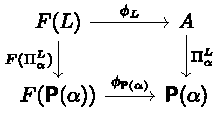
\includegraphics[width=0.95\linewidth,height=0.45\textheight,keepaspectratio]{graphic-01.pdf}\end{center}
    
Also, by condition (1), $\phi_{\boldsymbol{\mathsf{P}}(\alpha)}$ is an $\alpha$-isomorphism. Thus, by Remark 40 (Appendix C), $\phi_{L}$ is an $\alpha$-isomorphism since the three other sides of the diagram above are $\alpha$-isomorphisms.\par
 
% END S4.SS2.SSS0.P0.SPx1.p2
 
% BEGIN S4.SS2.SSS0.P0.SPx1.p3
 
The cone $\mathit{DCone}(\boldsymbol{\mathsf{P}})$ that we wish to show dominates $\boldsymbol{\mathsf{P}}$ is the following:\par
 
\begin{center}\resizebox{\linewidth}{!}{$\begin{aligned}\displaystyle\mathit{DCone}(\boldsymbol{\mathsf{P}})=\left((F(L),F(\phi_{L})),\left\{\phi_{\boldsymbol{\mathsf{P}}(\alpha)}\circ F(\Pi^{L}_{\alpha})\right\}_{\alpha\in A}\right)\end{aligned}$}\end{center}
 
We already established (1) when we argued that the diagram above consists of $\alpha$-isomorphisms. For (2), let us assume we are given an ordinal $\alpha$ for which we have $\left\{\beta\middle|\beta\prec\alpha\right\}\subseteq A$. We just observed that $\phi_{L}$ is an $A$-isomorphism and thus also a $\left\{\beta\middle|\beta\prec\alpha\right\}$-isomorphism. Hence, by Lemma 17 $F(\phi_{L})$ is an $\alpha$-isomorphism. $\hfill\blacktriangleleft$\par
 
% END S4.SS2.SSS0.P0.SPx1.p3
 
% BEGIN S4.SS2.SSS0.P0.SPx1.p4
 
Next we define what we call canonical partial solutions and show how to patch canonical partial solutions together in order to construct larger ones. The latter is used in Theorem 30 for constructing partial solutions by well-founded induction on ordinals.\par
 
% END S4.SS2.SSS0.P0.SPx1.p4
 
% BEGIN Thmtheorem27
 
\par\medskip\noindent\textbf{Definition 27 (Canonical Partial Solutions ).}\par
 
% BEGIN Thmtheorem27.p1
 
Let $A\subseteq\mathbf{Ord}$ be a downwards-closed subset of ordinals and $\boldsymbol{\mathsf{P}}$ an $A$-partial solution. We say $\boldsymbol{\mathsf{P}}$ is a canonical partial solution if it is constructed at all stages via the construction in Lemma 26. That is, if for any $\alpha\in A$ we have\par
 
\begin{center}\resizebox{\linewidth}{!}{$\begin{aligned}\displaystyle\left(\boldsymbol{\mathsf{P}}(\alpha),\left\{\boldsymbol{\mathsf{P}}_{\beta\preceq\alpha}\right\}_{\beta\preceq\alpha}\right)=\mathit{DCone}\left({\left.\boldsymbol{\mathsf{P}}\right|}_{\left\{\beta\middle|\beta\prec\alpha\right\}}\right)\end{aligned}$}\end{center}
 
are equal cones of the diagram ${\left.\boldsymbol{\mathsf{P}}\right|}_{\left\{\beta\middle|\beta\prec\alpha\right\}}$.\par
 
% END Thmtheorem27.p1
 
% END Thmtheorem27
 
% BEGIN Thmtheorem28
 
\par\medskip\noindent\textbf{Lemma 28 ().}\par
 
% BEGIN Thmtheorem28.p1
 
Let $\boldsymbol{\mathsf{P}}$ and $\boldsymbol{\mathsf{Q}}$ be two canonical $A$-partial solutions. We have $\boldsymbol{\mathsf{P}}=\boldsymbol{\mathsf{Q}}$ (as diagrams, i.e., functors).\par
 
% END Thmtheorem28.p1
 
% END Thmtheorem28
 
% BEGIN S4.SS2.SSS0.P0.SPx1.p5
 
On paper, the Lemma 28 above is proven through a simple argument by transfinite induction. However, as we will discuss in Section 5, it is far from obvious to mechanize.\par
 
% END S4.SS2.SSS0.P0.SPx1.p5
 
% BEGIN Thmtheorem29
 
\par\medskip\noindent\textbf{Lemma 29 ().}\par
 
% BEGIN Thmtheorem29.p1
 
Let $\left\{\boldsymbol{\mathsf{P}}^{\alpha}\right\}_{\alpha\in A}$ be a collection of canonical partial solutions indexed by some downwards-closed subset of ordinals $A$ such that $\boldsymbol{\mathsf{P}}^{\alpha}$ is a canonical $\left\{\beta\middle|\beta\preceq\alpha\right\}$-partial solution. We can construct a canonical $A$-partial solution $\boldsymbol{\mathsf{Q}}$ by patching the partial solutions $\left\{\boldsymbol{\mathsf{P}}^{\alpha}\right\}_{\alpha\in A}$ together. That is, we take $\boldsymbol{\mathsf{Q}}(\alpha):=\boldsymbol{\mathsf{P}}^{\alpha}(\alpha)$ and take $\boldsymbol{\mathsf{Q}}_{\beta\preceq\alpha}:=\boldsymbol{\mathsf{P}}^{\alpha}_{\beta\preceq\alpha}$.\par
 
% END Thmtheorem29.p1
 
% END Thmtheorem29
 
% BEGIN S4.SS2.SSS0.P0.SPx1.p6
 
Note that the proof, and even the well-formedness of the statement of Lemma 29 above depends on Lemma 28. In particular, note that $\boldsymbol{\mathsf{Q}}_{\beta\preceq\alpha}$ must be a morphism from $\boldsymbol{\mathsf{Q}}(\alpha)$ to $\boldsymbol{\mathsf{Q}}(\beta)$, or equivalently from $\boldsymbol{\mathsf{P}}^{\alpha}(\alpha)$ to $\boldsymbol{\mathsf{P}}^{\beta}(\beta)$, whereas the morphism $\boldsymbol{\mathsf{P}}^{\alpha}_{\beta\preceq\alpha}$ is a morphism from $\boldsymbol{\mathsf{P}}^{\alpha}(\alpha)$ to $\boldsymbol{\mathsf{P}}^{\alpha}(\beta)$. Thus, one would need to prove $\boldsymbol{\mathsf{P}}^{\alpha}(\beta)=\boldsymbol{\mathsf{P}}^{\beta}(\beta)$ for it to even make sense to take $\boldsymbol{\mathsf{Q}}_{\beta\preceq\alpha}:=\boldsymbol{\mathsf{P}}^{\alpha}_{\beta\preceq\alpha}$. This is the case because by Lemma 28 ${\left.\boldsymbol{\mathsf{P}}^{\alpha}\right|}_{\left\{\gamma\middle|\gamma\preceq\beta\right\}}=\boldsymbol{\mathsf{P}}^{\beta}$. However, in type theory, in our Rocq mechanization, one needs to work up to the equality $\boldsymbol{\mathsf{P}}^{\alpha}(\beta)=\boldsymbol{\mathsf{P}}^{\beta}(\beta)$ (transport along this equality) when defining $\boldsymbol{\mathsf{Q}}$, which also includes establishing its functoriality, that it is a partial solution, and its canonicity. We will discuss these subtleties in Section 5.\par
 
% END S4.SS2.SSS0.P0.SPx1.p6
 
% BEGIN Thmtheorem30
 
\par\medskip\noindent\textbf{Theorem 30 ().}\par
 
% BEGIN Thmtheorem30.p1
 
The locally contractive functor $F$ has a solution.\par
 
% END Thmtheorem30.p1
 
% END Thmtheorem30
 
% END S4.SS2.SSS0.P0.SPx1

% BEGIN Thmtheorem30
 
\par\medskip\noindent\textbf{Theorem 30 ().}\par
 
% BEGIN Thmtheorem30.p1
 
The locally contractive functor $F$ has a solution.\par
 
% END Thmtheorem30.p1
 
% END Thmtheorem30

 
% END S4.SS2.SSS0.P0.SPx1
 

% BEGIN S4.SS2.SSS0.P0.SPx2
 
\par\medskip\noindent\textbf{Proof.}\par
 
% BEGIN S4.SS2.SSS0.P0.SPx2.p1
 
We first construct a canonical $\mathbf{Ord}$-partial solution $\boldsymbol{\mathsf{P}}$. By Lemma 29 it suffices to construct canonical $\left\{\beta\middle|\beta\preceq\alpha\right\}$-partial solutions for all $\alpha\in\mathbf{Ord}$. We do so by well-founded induction on $\alpha$. Thus, let us assume that we have canonical $\left\{\gamma\middle|\gamma\preceq\beta\right\}$-partial solutions for all $\beta\prec\alpha$. We use Lemma 29 to construct a canonical $\left\{\beta\middle|\beta\preceq\alpha\right\}$-partial solution as required. The solution is the $F$-algebra of $\mathit{DCone}(\boldsymbol{\mathsf{P}})$. We only need to show that the map $\phi_{\mathit{DCone}(\boldsymbol{\mathsf{P}})}$ is an isomorphism. By Lemma 15 it suffices to show that $\phi_{\mathit{DCone}(\boldsymbol{\mathsf{P}})}$ is an $\alpha$-isomorphism for all $\alpha\in\mathbf{Ord}$. However, by Lemma 26 $\mathit{DCone}(\boldsymbol{\mathsf{P}})$ dominates $\boldsymbol{\mathsf{P}}$. Hence, by the property (2) of dominating cones we only need to show that $\left\{\beta\middle|\beta\prec\alpha\right\}\subseteq\mathbf{Ord}$, which holds trivially. $\hfill\blacktriangleleft$\par
 
% END S4.SS2.SSS0.P0.SPx2.p1
 
% BEGIN Thmtheorem31
 
\par\medskip\noindent\textbf{$\blacktriangleright$ Remark 31.}\par
 
% BEGIN Thmtheorem31.p1
 
In addition to the difference of working with the category of $F$-algebras as opposed to working directly in $\mathcal{C}$, our approach to solving domain equations differs from that presented by Birkedal et al. [9] in how we treat zero and limit ordinals. Working with sheaves, Birkedal et al. [9] at zero and limit ordinals simply take the limit of the construction at stages below. By contrast, we apply $F$ to the obtained cone of the limit at every single stage of the construction and not just at successor ordinals. Another way to look at this difference is if we look at the sequence of objects constructed in these two approaches (in our case the carrier objects of the algebras we compute). Up to isomorphism, what we compute is the sequence $X$ below while what Birkedal et al. [9] compute is the sequence $Y$:      $\displaystyle X_{0}:={}$ $\displaystyle F(1);$ $\displaystyle X_{1}:={}$ $\displaystyle F(F(1));$ $\displaystyle X_{2}:={}$ $\displaystyle F(F(F(1)));$ $\displaystyle\cdots$ $\displaystyle X_{\omega}:={}$ $\displaystyle F(\lim_{\alpha\prec\omega}X_{\alpha});$ $\displaystyle X_{{\omega}^{+}}:={}$ $\displaystyle F(X_{\omega});$ $\displaystyle\cdots$    $\displaystyle Y_{0}:={}$ $\displaystyle 1;$ $\displaystyle Y_{1}:={}$ $\displaystyle F(1);$ $\displaystyle Y_{2}:={}$ $\displaystyle F(F(1));$ $\displaystyle\cdots$ $\displaystyle Y_{\omega}:={}$ $\displaystyle\lim_{\alpha\prec\omega}Y_{\alpha};$ $\displaystyle Y_{{\omega}^{+}}:={}$ $\displaystyle F(Y_{\omega});$ $\displaystyle\cdots$\par
 
% END Thmtheorem31.p1
 
% END Thmtheorem31
 
% END S4.SS2.SSS0.P0.SPx2

 
% END S4.SS2
 
% BEGIN S4.SS3
 
\par\medskip\noindent\textbf{4.3 Mixed-Variance Domain Equations}\par
 
% BEGIN S4.SS3.p1
 
In addition to covariant functors of the form $\mathcal{C}\to\mathcal{C}$, we in general need to [9] solve domain equations for mixed-variance functors of the form ${\mathcal{C}}^{\mathsf{op}}\times\mathcal{C}\to\mathcal{C}$.\par
 
% END S4.SS3.p1
 
% BEGIN Thmtheorem32
 
\par\medskip\noindent\textbf{Example 32 ().}\par
 
% BEGIN Thmtheorem32.p1
 
As a simple minimal example we have used our development to solve the domain equation for the following mixed-variance functor which is a simplified version of the functor used by Frumin et al. [17]:\par
 
\begin{center}\resizebox{\linewidth}{!}{$\begin{aligned}\displaystyle F(X,Y):=\Delta(\mathbb{N})+\mathop{\blacktriangleright}(Y^{X})+\mathop{\blacktriangleright}Y\end{aligned}$}\end{center}
 
where $\Delta(A)$ is the constant presheaf mapping all ordinals to the set $A$.\par
 
% END Thmtheorem32.p1
 
% END Thmtheorem32
 
% BEGIN S4.SS3.p2
 
The following lemma shows that mixed-variance locally contractive functors $F:{\mathcal{C}}^{\mathsf{op}}\times\mathcal{C}\to\mathcal{C}$ like the one in Example 32 have unique solutions.\par
 
% END S4.SS3.p2
 
% BEGIN Thmtheorem33
 
\par\medskip\noindent\textbf{Lemma 33 ().}\par
 
% BEGIN Thmtheorem33.p1
 
Let $\mathcal{C}$ be a $\mathbf{PSh}(\mathbf{Ord})$-enriched category and $F:{\mathcal{C}}^{\mathsf{op}}\times\mathcal{C}\to\mathcal{C}$ be a locally contractive functor (if $\mathcal{C}$ is enriched, so is ${\mathcal{C}}^{\mathsf{op}}$ and also their product). Furthermore, assume that $\mathcal{C}$ is complete and co-complete with enriched-pointwise limits and co-limits. The functor $F$ has a unique solution.\par
 
% END Thmtheorem33.p1
 
% END Thmtheorem33
 
% BEGIN S4.SS3.SSS0.P0.SPx1
 
\par\medskip\noindent\textbf{Proof.}\par
 
% BEGIN S4.SS3.SSS0.P0.SPx1.p1
 
Define the functor $\tilde{F}(A,B):=(F(B,A),F(A,B))$ from ${\mathcal{C}}^{\mathsf{op}}\times\mathcal{C}$ to ${\mathcal{C}}^{\mathsf{op}}\times\mathcal{C}$. The functor $\tilde{F}$ is also locally contractive and hence, by Theorem 30, has a solution, say $(X,Y)$ for which $\tilde{F}(X,Y)\simeq(X,Y)$. In that case, by symmetry of $\tilde{F}$, we have $\tilde{F}(Y,X)\simeq(Y,X)$. Thus, by Theorem 23, $(X,Y)\simeq(Y,X)$ which implies that $X\simeq Y$, and hence, $F(X,X)\simeq X$. $\hfill\blacktriangleleft$\par
 
% END S4.SS3.SSS0.P0.SPx1.p1
 
% END S4.SS3.SSS0.P0.SPx1
 
% END S4.SS3
 
% END S4


% BEGIN S5
 
\par\medskip\noindent\textbf{5 Rocq Mechanization}\par
 
% BEGIN S5.p1
 
All results that have been marked by a  symbol throughout the paper and the appendices are mechanized [46] in the Rocq Prover. For this mechanization we have used the step-indexing interface of Spies et al. [45] which abstracts a step-indexing structure that Spies et al. [45] instantiate twice: once with natural numbers in Rocq (for step-indexing over $\omega$), and once with ordinal numbers. Spies et al. [45] use the mechanization of ordinal numbers by Kirst et al. [31]. We use the following axioms in our mechanization: axiom of choice (and its consequence excluded middle), propositional extensionality (and its consequences proof irrelevance and uniqueness of identity proofs (UIP)), and functional extensionality. The first two of these axioms are already assumed by Kirst et al. [31] to construct a model of set theory in Rocq. The inclusion of functional extensionality, on the other hand, is necessary for formalization of category theory, at least the way we have; we will discuss this below.\par
 
% END S5.p1
 
% BEGIN S5.SS0.SSS0.P0.SPx1
 
\par\medskip\noindent\textbf{The Notion of Equality of Homorphisms in Type Theory.}\par
 
% BEGIN S5.SS0.SSS0.P0.SPx1.p1
 
There are many efforts mechanizing category theory in type-theory-based proof assistants [24, 40, 25, 52, 21, 49, 50, 2, 36]. Hu and Carette [24] give an extensive survey comparing existing type-theory-based category theory mechanizations across multiple different axes. One important design point in mechanizing category theory in type theory is representing equality of morphisms. Roughly speaking, this design decision divides mechanizations into two camps: those using setoids, also known as Bishop sets [12], for representing morphisms [24, 40, 25, 52] and those using equality [21, 49, 50, 2, 36] (including those working in HoTT [50] settings where equality plays a key role).\par
 
% END S5.SS0.SSS0.P0.SPx1.p1
 
% BEGIN S5.SS0.SSS0.P0.SPx1.p2
 
There are multiple advantages to using setoids as pointed out by Hu and Carette [24]. Hu and Carette [24] work in Agda and state “Our principal theoretical contribution is to show that setoid-based proof-relevant category theory works just as well as various other “flavours” of category theory by supporting a large number of definitions and theorems.” One of the main advantages of using setoids is avoiding axioms such as functional extensionality (for proving equality of functors, natural transformations, etc.) and classical axioms (for constructing quotient types, e.g., for co-limits in $\mathbf{Set}$ or presheaf categories) – of course, works based in HoTT admit these as theorems. Indeed, our development also started with implementing the necessary basic concepts in category theory using setoids. However, we discovered an issue that fundamentally precludes the use of setoids for morphisms in our mechanization. This problem arises in the proof of Lemma 28. For this lemma, we need to show that two $F$-algebras are equal which are constructed based on the limits of two diagrams that are equal (by our transfinite induction hypothesis). However, the natural notion of equality of functors in setoid settings is to ask that the morphism maps of functors map setoid-equal morphisms into setoid-equal morphisms. Consequently, the best one can prove is that equal functors in this sense produce isomorphic limits. Thus, instead of Lemma 28, one could prove that canonical partial solutions are naturally isomorphic. However, as remarked after Lemma 29 in Section 4.2, this is not even sufficient for the statement of Lemma 29 to be well-formed. This is why we chose to change our mechanization to use the equality notion from Rocq’s standard library instead of setoid equality. It appears that existing mechanizations of category theory that formalize collections of morphisms as setoids have never attempted formalizing a construction such as ours that involves defining a functor on ordinals by transfinite induction where the construction at each stage involves taking the limit of the construction up to below that stage.\par
 
% END S5.SS0.SSS0.P0.SPx1.p2
 
% END S5.SS0.SSS0.P0.SPx1
 
% BEGIN S5.SS0.SSS0.P0.SPx2
 
\par\medskip\noindent\textbf{Working With All Ordinals in The Universe.}\par
 
% BEGIN S5.SS0.SSS0.P0.SPx2.p1
 
As we discussed in the Introduction, we work with the category of presheaves over all ordinals in the universe, i.e., the set $\mathbf{Ord}$ which is not closed under suprema. Thus, many of our definitions are parameterized by a downwards-closed subset of ordinals. The collection of downwards-closed subsets of ordinals, ordered by the subset relation, can be thought of as the ideal completion of $\mathbf{Ord}$. In particular, the total set $\mathbf{Ord}$ is the maximal element of this order which represents the supremum of the entire set $\mathbf{Ord}$. This means that the key lemma of our formalization, Lemma 29, is applicable to both proper downwards-closed subsets of ordinals (which represent ordinals that do happen to be in $\mathbf{Ord}$) as well as the aforementioned supremum of the entire set $\mathbf{Ord}$ (which itself is not in $\mathbf{Ord}$). This is why we can apply Lemma 29 twice in the proof of Theorem 30, once for constructing $\left\{\beta\middle|\beta\preceq\alpha\right\}$-partial solutions for all $\alpha\in\mathbf{Ord}$ by transfinite induction on $\alpha$, and once to put all those together to construct a $\mathbf{Ord}$-partial solution. This is key in significantly reducing the size of the mechanization as otherwise a mechanization working with all ordinals in the universe would have to prove two different versions of Lemma 29 for the two different use cases in Theorem 30; once for individual ordinals, and once for all ordinals. Spies et al. [45] also work with the collection of ordinals in the universe; as mentioned above we took their notion of step-indexing and ordinals verbatim in our mechanization. And, they indeed duplicate Lemma 29 as we just explained. This requires them to repeat multiple definitions and lemmas for these two versions of our single Lemma 29.\par
 
% END S5.SS0.SSS0.P0.SPx2.p1
 
% END S5.SS0.SSS0.P0.SPx2
 
% BEGIN S5.SS0.SSS0.P0.SPx3
 
\par\medskip\noindent\textbf{Well-Behaved Subset Types in Rocq.}\par
 
% BEGIN S5.SS0.SSS0.P0.SPx3.p1
 
Working with downwards-closed subsets of ordinals, we need to formalize them in our Rocq mechanization. In our mechanization, we define downwards-closed subsets of ordinals as subset types which we represent as a record that packages an ordinal together with a proof that said ordinal is in the downwards-closed subset. We first define downwards-closed predicates over ordinals, downset\_pred, as a record type consisting of a predicate together with a proof that this predicate is downwards-closed (ignore the decidability part for now, we will get back to it):\par
  \ensuremath{\downarrow} 
% BEGIN lstnumberx1
 Polymorphic Record downset\_pred (SI : indexT) := MkDownSetPred \{ 
% END lstnumberx1
 
% BEGIN lstnumberx2
  dsp\_pred :> SI → Prop; 
% END lstnumberx2
 
% BEGIN lstnumberx3
  dsp\_pred\_dec : \ensuremath{\forall} \ensuremath{\alpha}, Decision (dsp\_pred \ensuremath{\alpha}); 
% END lstnumberx3
 
% BEGIN lstnumberx4
  dsp\_pred\_downwards : \ensuremath{\forall} \ensuremath{\alpha} \ensuremath{\beta}, \ensuremath{\alpha} \ensuremath{\preceq} \ensuremath{\beta} → dsp\_pred \ensuremath{\beta} → dsp\_pred \ensuremath{\alpha}; \}. 
% END lstnumberx4
  
Here, indexT is the generalized type exposed by the step-indexing interface of Spies et al. [45]; the type of all ordinals in the universe being an instance of this structure. Based on the downwards-closed predicates defined above, we would like to define downwards-closed subsets essentially as a record type that packages together an ordinal, together with a proof that it belongs to the provided downwards-closed predicate. However, a naïve encoding as such a record type leads to a problem: given a downwards-closed predicate over ordinals, two elements of such a type with the same ordinals but different proofs would not be definitionally equal – of course, they are propositionally equal as we assume proof irrelevance. This problem is especially noticeable when we look at two downwards-closed subsets where one is included in the other. We define the inclusion relation between two downwards-closed predicates dsp and dsp’ as one would expect: \ensuremath{\forall} \ensuremath{\alpha}, dsp \ensuremath{\alpha} → dsp’ \ensuremath{\alpha}. This allows us to define a simple function that lifts ordinals from the smaller downwards-closed subset to the larger one. We use this function in our Rocq mechanization to define the restriction operation in Section 4.2 on presheaves over downwards-closed subsets of ordinals.\par
 
% END S5.SS0.SSS0.P0.SPx3.p1
 
% BEGIN S5.SS0.SSS0.P0.SPx3.p2
 
We solve the issue discussed above by defining the record type downset as follows:\par
  \ensuremath{\downarrow} 
% BEGIN lstnumberx5
 \#[projections(primitive = yes)] 
% END lstnumberx5
 
% BEGIN lstnumberx6
 Record downset \{SI\} (dsp : downset\_pred SI) := MkDS \{ 
% END lstnumberx6
 
% BEGIN lstnumberx7
  ds\_idx :> SI; 
% END lstnumberx7
 
% BEGIN lstnumberx8
  ds\_in\_dsp : squashed (dsp ds\_idx); \}. 
% END lstnumberx8
  
where the type squashed is exactly as defined in Gilbert et al. [20]:\par
  \ensuremath{\downarrow} 
% BEGIN lstnumberx9
 Inductive squashed (P : Prop) : SProp := squash : P → squashed P. 
% END lstnumberx9
  
The idea here is that since squashed is in the universe SProp of definitionally proof-irrelevant propositions, and the fact that type downset is defined as a record with primitive projections (and hence it is subject to the $\eta$ conversion law for records), two terms of the type downset dsp are definitionally equal as soon as their underlying ordinal, the projection ds\_idx, are definitionally equal. Now, the problem is that when working with elements of downset dsp, we need to have a proof that the underlying ordinal is indeed in dsp, i.e., we need something of type dsp ds\_idx, whereas we are only given a proof of squashed (dsp ds\_idx). Importantly, the type squashed above cannot be eliminated to produce a term of a type that is outside the universe SProp – in technical terms, this is because the first argument of the constructor squash (the argument with type P) is non-forced, and is also not in SProp [20]. Nevertheless, inspired by the constant map from identity proofs to identity proofs in the proof of Hedberg’s theorem [23], we prove the following lemma which allows us to recover a proof of dsp ds\_idx from an element of squashed (dsp ds\_idx):444Gilbert et al. [20] use the name unsquash for the eliminator of their squashed type (which they call squash, and its constructor sq) that only eliminates into other SProp types.\par
  \ensuremath{\downarrow} 
% BEGIN lstnumberx10
 Lemma unsquash \{P : Prop\} ‘\{!Decision P\} (s : squashed P) : P. 
% END lstnumberx10
  
The lemma above is the reason why we included a proof of decidability of the subset predicate in the definition of downset\_pred above.\par
 
% END S5.SS0.SSS0.P0.SPx3.p2
 
% END S5.SS0.SSS0.P0.SPx3
 
% END S5


% BEGIN S6
 
\par\medskip\noindent\textbf{6 Related Works}\par
 
% BEGIN S6.SS0.SSS0.P0.SPx1
 
\par\medskip\noindent\textbf{Domain Theory.}\par
 
% BEGIN S6.SS0.SSS0.P0.SPx1.p1
 
We have already discussed works on domain theory that are most closely related to ours in the Introduction, including the most closely related work to ours [9] which our work is closely based on, and which we have compared our work to throughout the paper.\par
 
% END S6.SS0.SSS0.P0.SPx1.p1
 
% END S6.SS0.SSS0.P0.SPx1
 
% BEGIN S6.SS0.SSS0.P0.SPx2
 
\par\medskip\noindent\textbf{Fixed Points in Type Theory.}\par
 
% BEGIN S6.SS0.SSS0.P0.SPx2.p1
 
When working with inductive and co-inductive types and proofs in type theory, it is required to follow restrictive syntactic checks (e.g., productivity and guardedness for co-induction). These overly strong syntactic conditions protect mechanizations against inconsistencies, but reject many valid definitions. Motivated alleviate this situation, Di Gianantonio and Miculan [18] introduce complete ordered families of equivalences (COFEs) as a unifying theory for mixed-variance recursive definitions that support construction of fixed points. They define COFEs over an arbitrary well-founded order and prove a generalized fixed point theorem for contractive endofunctions over these COFEs. In a subsequent work, Di Gianantonio and Miculan [19] generalize this result to sheaf categories over topologies with a well-founded basis – this is very close to the setting of Birkedal et al. [9] upon which we have based our work. The main difference between the works of Di Gianantonio and Miculan [18, 19] and Birkedal et al. [9], and thereby also our work, is that the former only constructs fixed points of morphisms (similar to our results in Section 2.2) whereas the latter also constructs fixed points of functors.\par
 
% END S6.SS0.SSS0.P0.SPx2.p1
 
% END S6.SS0.SSS0.P0.SPx2
 
% BEGIN S6.SS0.SSS0.P0.SPx3
 
\par\medskip\noindent\textbf{Mechanizations of Solutions to Domain Equations.}\par
 
% BEGIN S6.SS0.SSS0.P0.SPx3.p1
 
Benton et al. [6] mechanize solution to domain equations over directed-complete partial orders (DCPOs) in the Rocq Prover based on the mechanization of DCPOs by Paulin-Mohrig [38]. Huffman [26] constructs a universal domain into which all bifinite domains can be embedded. Dockins [15] mechanizes solutions of domain equations over the category of profinite domains [22] in Rocq. All these works are based on classical domain theory, and as also pointed out by Sieczkowski et al. [43], unlike our guarded domains, do not appear to be suitable for modeling higher-order program logics like Iris [29].\par
 
% END S6.SS0.SSS0.P0.SPx3.p1
 
% BEGIN S6.SS0.SSS0.P0.SPx3.p2
 
The most closely related works to us are Rocq mechanizations of the domain equation solver of the ModuRes library [43], the domain equation solver of the Iris program logic [28] which is a nicer reimplementation of the domain equation solver of the ModuRes library, and the domain equation solver of transfinite Iris [45]. The former two mechanizations work with the category of COFEs (these are COFEs over $\omega$ and not over an arbitrary ordered set like Di Gianantonio and Miculan [18]), a representation of the category of complete bisected bounded ultra metric spaces (CBUlt) [11] that is particularly amenable to mechanizations [43]. These works only support step-indexing up to $\omega$. Transfinite Iris, inspired by Birkedal et al. [9], extend the definition of OFEs (COFEs without completeness requirement) and COFEs over $\omega$ to those over $\mathbf{Ord}$. However, Transfinite Iris, unlike the ModuRes library and Iris, only solves domain equations for functors of the form ${\mathrm{OFE}}^{\mathsf{op}}\times\mathrm{OFE}\to\mathrm{COFE}$ and not ${\mathrm{COFE}}^{\mathsf{op}}\times\mathrm{COFE}\to\mathrm{COFE}$. An example of a functor that is not supported by transfinite Iris as a result of this limitation is our Example 32.\par
 
% END S6.SS0.SSS0.P0.SPx3.p2
 
% END S6.SS0.SSS0.P0.SPx3
 
% BEGIN S6.SS0.SSS0.P0.SPx4
 
\par\medskip\noindent\textbf{Mechanizations of Category Theory.}\par
 
% BEGIN S6.SS0.SSS0.P0.SPx4.p1
 
We mentioned the existing mechanizations of category theory in Section 5. We refer to Hu and Carette [24] who give an extensive survey comparing these mechanizations. Regarding our mechanization of category theory, we only mention that its span is not significant compared to the works cited, compared, and contrasted by Hu and Carette [24]. We have only mechanized what was necessary for formalizing our main results: Theorem 23, Theorem 30 and Lemma 33.\par
 
% END S6.SS0.SSS0.P0.SPx4.p1
 
% END S6.SS0.SSS0.P0.SPx4
 
% END S6


% BEGIN S7
 
\par\medskip\noindent\textbf{7 Future Work}\par
 
% BEGIN S7.p1
 
Our main future goal is to build a step-indexed (program) logic similar to the Iris framework [29] based on our development. We hope to use such a step-indexed logic to study weak bisimulation of guarded interaction trees, i.e., objects similar to the one shown in Example 32. This requires transfinite step-indexing because we need to allow either side of the bisimulation relation to take finitely many silent steps ($\tau$-steps). However, as we discussed in Section 6, the existing work on transfinite step-indexing does not support equations like that in Example 32. However, there is a significant amount of nontrivial technical work that needs to be done before we can put our mechanization to use for constructing a user-friendly step-indexed (program) logic framework, e.g., providing an interactive proof mode similar to that of the Iris framework [33, 32]. In principle, the main limiting factor is the complexity of working with presheaves compared to COFEs in proof assistants; using our solution forces one to always use categories and categorical constructions. For instance, maps between COFEs are non-expansive functions (Rocq functions with a side-condition), while maps between presheaves are natural transformations (families of functions with a naturality side-condition relating these families). Thus, while presheaves are more amenable to mechanization than sheaves, there remains a substantial amount of work required to build a user-friendly (program) logic framework on top of our category theoretic development. This makes developing a user-friendly system on top of our development very challenging, which we leave as an important future work.\par
 
% END S7.p1
 
% END S7


% BEGIN S8
 
\par\medskip\noindent\textbf{8 Conclusion}\par
 
% BEGIN S8.p1
 
After motivating the need for solving domain equations over the category of presheaves over ordinals, we presented the theory of solving such domain equations and discussed its mechanization as well as the challenges we faced mechanizing this theory. As demonstrated by our Example 32, this domain equation solver can be used to solve domain equations stated as mixed-variance functors like those that are needed for guarded interaction trees [17] or program logics [45].\par
 
% END S8.p1
 
% END S8


% BEGIN A1
 
\par\medskip\noindent\textbf{Appendix A The Need for Step-Indexing Over Higher Ordinals}\par
 
% BEGIN A1.p1
 
As we discussed in the Introduction, the main issue is that when working with step-indexing over $\omega$ the existential property fails to hold. That is, if we know that $\models\exists x:A.\;\phi(x)$ holds, we do necessarily get that there exists an $a\in A$ such that $\models\phi(a)$ holds. In this appendix, we first discuss why the existential property fails when step-indexing over $\omega$. We then present a proof for a general criterion of when the existential property does hold, and based on this criterion motivate our choice (and that of Spies et al. [45]) to use step-indexing over all ordinals in a Grothendieck universe.\par
 
% END A1.p1
 
% BEGIN A1.SS1
 
\par\medskip\noindent\textbf{A.1 Failure of the Existential Property}\par
 
% BEGIN A1.SS1.p1
 
Recall that in step-indexing over $\omega$ the set of truth values is the Heyting algebra of the downwards-closed subsets of $\omega$. In this setting, the interpretation of $\phi$, $\left\llbracket\phi\right\rrbracket$, is a function from $A$ into this Heyting algebra, and we have $\left\llbracket\exists x:A.\;\phi(x)\right\rrbracket=\bigcup_{x\in A}\left\llbracket\phi\right\rrbracket(x)$. Thus, $\models\exists x:A.\;\phi(x)$ is equivalent to saying that $\bigcup_{x\in A}\left\llbracket\phi\right\rrbracket(x)=\omega$, i.e., that the interpretation of $\exists x:A.\;\phi(x)$ is the truth value $\top$, which in our Heyting algebra is the entire set $\omega$. Now, take $A:=\mathbb{N}$ and $\phi(n):=\rhd^{n}\bot$. Readers not familiar with step-indexed logics can ignore the exact definition of $\phi$. (These readers are kindly referred to Jung et al. [29] for a detailed explanation of the syntax and semantics of the step-indexed logic Iris). What is important for us is that $\left\llbracket\rhd^{n}\bot\right\rrbracket=\left\{k\middle|k<n\right\}$. Based on this interpretation one can easily see that $\bigcup_{n\in\mathbb{N}}\left\llbracket\rhd^{n}\bot\right\rrbracket=\omega$ but there is no $n\in\mathbb{N}$ such that $\left\llbracket\rhd^{n}\bot\right\rrbracket=\omega$.\par
 
% END A1.SS1.p1
 
% END A1.SS1
 
% BEGIN A1.SS2
 
\par\medskip\noindent\textbf{A.2 A General Criterion for the Existential Property to Hold}\par
 
% BEGIN A1.SS2.p1
 
Here, we present a general criterion of when the universal property holds. This section is based on a blog post by the second author [48].\par
 
% END A1.SS2.p1
 
% BEGIN Thmtheorem34
 
\par\medskip\noindent\textbf{Theorem 34 ().}\par
 
% BEGIN Thmtheorem34.p1
 
If the step-indexing is a regular ordinal and the cardinality of the set quantified over is strictly smaller than that of the step-indexing ordinal, then the existential property holds.\par
 
% END Thmtheorem34.p1
 
% END Thmtheorem34
 
% BEGIN Thmtheorem35
 
\par\medskip\noindent\textbf{$\blacktriangleright$ Remark 35.}\par
 
% BEGIN Thmtheorem35.p1
 
The Rocq mechanization of Theorem 34 does not use ordinals or a step-indexed logic. It follows very closely the ideas in the blog post [48]. It first defines an analogue of regularity for an arbitrary Rocq type $A$ with a relation $R\subseteq A\times A$ on it. Then, it shows that $\forall a:A.\;\exists b:B.\;P(a,b)$ implies $\exists b:B.\;\forall a:A.\;P(a,b)$ whenever the type $A$ is regular, the cardinality of $B$ is strictly smaller than that of $A$, and furthermore $P$ is downwards-closed with respect to $R$, i.e., if $\forall a,a^{\prime}\in A,b\in B.\;R(a,a^{\prime})\land P(a^{\prime},b)\implies P(a,b)$.\par
 
% END Thmtheorem35.p1
 
% END Thmtheorem35
 
% BEGIN A1.SS2.p2
 
Below, we first give the definition of regular ordinals (which can be found in most standard textbooks on set theory [27]) and then give the proof of Theorem 34.\par
 
% END A1.SS2.p2
 
% BEGIN Thmtheorem36
 
\par\medskip\noindent\textbf{Definition 36.}\par
 
% BEGIN Thmtheorem36.p1
 
We say an ordinal $\gamma$ is regular, if the supremum of any sequence of ordinals strictly smaller than $\gamma$, indexed by an ordinal strictly smaller than $\gamma$, is also strictly smaller than $\gamma$. In other words, for any sequence of ordinals $\left\{\beta_{\alpha}\right\}_{\alpha\preceq\delta}$ indexed by an ordinal $\delta$, if we have both that $\delta\prec\gamma$, and that $\forall\alpha\preceq\delta.\;\beta_{\alpha}\prec\gamma$, then $\bigcup_{\alpha\preceq\delta}\beta_{\alpha}\prec\gamma$.\par
 
% END Thmtheorem36.p1
 
% END Thmtheorem36
 
% BEGIN A1.SS2.SSS0.P0.SPx1
 
\par\medskip\noindent\textbf{Proof of Theorem 34.}\par
 
% BEGIN A1.SS2.SSS0.P0.SPx1.p1
 
Let us assume that we are working with a logic step-indexed over a regular ordinal $\gamma$ – thus, the set of truth values is the Heyting algebra of downwards-closed subsets of $\gamma$. Furthermore, let us assume we are given a set $A$ whose cardinality is strictly smaller than that of $\gamma$. (More specifically, let us assume that $A=\left\{a_{\alpha}\middle|\alpha\preceq\delta\right\}$ for some $\delta\prec\gamma$.) Finally, assume we are given a predicate $\phi$ over $A$ such that $\left\llbracket\exists x:A.\;\phi(x)\right\rrbracket=\bigcup_{x\in A}\left\llbracket\phi\right\rrbracket(x)=\gamma$. We show, using proof by contradiction, that there exists an element $a\in A$ such that $\left\llbracket\phi\right\rrbracket(a)=\gamma$.\par
 
% END A1.SS2.SSS0.P0.SPx1.p1
 
% BEGIN A1.SS2.SSS0.P0.SPx1.p2
 
Assume, to the contrary that there is no element $a\in A$ such that $\left\llbracket\phi\right\rrbracket(a)=\gamma$. In other words, for any $a\in A$ there is an ordinal $\beta\prec\gamma$ such that $\beta\not\in\left\llbracket\phi\right\rrbracket(a)$. Now, since $A=\left\{a_{\alpha}\middle|\alpha\preceq\delta\right\}$, this forms a sequence of ordinals $\left\{\beta_{\alpha}\right\}_{\alpha\preceq\delta}$ such that $\forall\alpha\preceq\delta.\;\beta_{\alpha}\prec\gamma$ and that $\forall\alpha\preceq\delta.\;\beta_{\alpha}\not\in\left\llbracket\phi\right\rrbracket(a_{\alpha})$. Thus, by regularity of $\gamma$, we have that $\bigcup_{\alpha\preceq\delta}\beta_{\alpha}\prec\gamma$, and by the fact that for any $a$ the set $\left\llbracket\phi\right\rrbracket(a)$ is downwards-closed, we have that $\forall\alpha\preceq\delta.\;\bigcup_{\alpha\preceq\delta}\beta_{\alpha}\not\in\left\llbracket\phi\right\rrbracket(a_{\alpha})$. Hence, it must be the case that $\bigcup_{\alpha\preceq\delta}\beta_{\alpha}\not\in\bigcup_{\alpha\preceq\delta}\left\llbracket\phi\right\rrbracket(a_{\alpha})=\bigcup_{x\in A}\left\llbracket\phi\right\rrbracket(x)=\left\llbracket\exists x:A.\;\phi(x)\right\rrbracket$, which is a contradiction. $\hfill\blacktriangleleft$\par
 
% END A1.SS2.SSS0.P0.SPx1.p2
 
% BEGIN A1.SS2.SSS0.P0.SPx1.p3
 
We remark that the set of all ordinals in the universe acts basically as a regular ordinal – indeed, this must be understood as step-indexing over the supremum of that set which is regular. In other words, we have by definition that for any function $A\to\mathbf{Ord}$ where $A$ is a set/type in the universe, the supremum of the image of the function is again an ordinal in $\mathbf{Ord}$. Thus, when step-indexing over all ordinals in the universe, by Theorem 34, we get that the existential property holds for quantification over any set in the universe.\par
 
% END A1.SS2.SSS0.P0.SPx1.p3
 
% END A1.SS2.SSS0.P0.SPx1
 
% END A1.SS2
 
% END A1


% BEGIN A2
 
\par\medskip\noindent\textbf{Appendix B Later is Locally Contractive, Earlier is not Even Enriched}\par
 
% BEGIN Thmtheorem37
 
\par\medskip\noindent\textbf{Theorem 37 (Later is Enriched and Locally Contractive ).}\par
 
% BEGIN Thmtheorem37.p1
 
The functor $\mathop{\blacktriangleright}:\mathbf{PSh}(\mathbf{Ord})\to\mathbf{PSh}(\mathbf{Ord})$ is an enriched and locally contractive functor.\par
 
% END Thmtheorem37.p1
 
% END Thmtheorem37
 
% BEGIN Thmtheorem38
 
\par\medskip\noindent\textbf{$\blacktriangleright$ Remark 38 (Earlier is not Enriched).}\par
 
% BEGIN Thmtheorem38.p1
 
The category $\mathbf{PSh}(\mathbf{Ord})$ is enriched over itself. Hence, we can ask whether the functor $\mathop{\blacktriangleleft}:\mathbf{PSh}(\mathbf{Ord})\to\mathbf{PSh}(\mathbf{Ord})$ is an enriched functor? The answer is negative. Here we give an intuitive explanation as to why this is not the case. We will formally prove this negative answer in Lemma 39.\par
 
% END Thmtheorem38.p1
 
% BEGIN Thmtheorem38.p2
 
To understand why earlier is not enriched note that we need to produce a natural transformation for the internal action of the earlier functor. That is, a natural transformation $G^{F}\to\mathop{\blacktriangleleft}G^{\mathop{\blacktriangleleft}F}$. By adjunction of exponentiation it is the same as requiring a natural transformation $G^{F}\times{\mathop{\blacktriangleleft}F}\to\mathop{\blacktriangleleft}G$. Let us look at an arbitrary component of this natural transformation at stage $\alpha$. That is, a function (morphism in $\mathbf{Set}$) $(\mathcal{Y}_{\alpha}\times F\to G)\times F({\alpha}^{+})\to G({\alpha}^{+})$. Such a map, given a natural transformation $\eta:\mathcal{Y}_{\alpha}\times F\to G$ and an element $x\in F({\alpha}^{+})$ must produce a an element of $G({\alpha}^{+})$. The only possibility here is to use $\eta_{{\alpha}^{+}}:\mathcal{Y}_{\alpha}({\alpha}^{+})\times F({\alpha}^{+})\to G({\alpha}^{+})$. However, set $\mathcal{Y}_{\alpha}({\alpha}^{+})=\left\{*\middle|{\alpha}^{+}\preceq\alpha\right\}$ is empty.\par
 
% END Thmtheorem38.p2
 
% END Thmtheorem38
 
% BEGIN A2.p1
 
As a simple corollary of uniqueness of solutions for locally contractive functors we prove that the functor earlier cannot be an enriched functor.\par
 
% END A2.p1
 
% BEGIN Thmtheorem39
 
\par\medskip\noindent\textbf{Lemma 39.}\par
 
% BEGIN Thmtheorem39.p1
 
The functor $\mathop{\blacktriangleleft}:\mathbf{PSh}(\mathbf{Ord})\to\mathbf{PSh}(\mathbf{Ord})$ is not an enriched functor for the self-enrichment of the category $\mathbf{PSh}(\mathbf{Ord})$.\par
 
% END Thmtheorem39.p1
 
% END Thmtheorem39
 
% BEGIN A2.SS0.SSS0.P0.SPx1
 
\par\medskip\noindent\textbf{Proof.}\par
 
% BEGIN A2.SS0.SSS0.P0.SPx1.p1
 
Assume that $\mathop{\blacktriangleleft}$ is an enriched functor. In that case, by Lemma 12 the functor $\mathop{\blacktriangleleft}\circ\mathop{\blacktriangleright}$ would be a locally contractive functor as $\mathop{\blacktriangleright}$ is by Lemma 37. However, the functor $\mathop{\blacktriangleleft}\circ\mathop{\blacktriangleright}$ is naturally isomorphic to $\mathsf{id}_{\mathbf{PSh}(\mathbf{Ord})}$. Recall that the co-unit of the adjunction $\mathop{\blacktriangleleft}\dashv\mathop{\blacktriangleright}$ is a natural isomorphism. Hence, any presheaf is a solution for the locally contractive functor $\mathop{\blacktriangleleft}\circ\mathop{\blacktriangleright}$, i.e., for any presheaf $F$ we have $\mathop{\blacktriangleleft}(\mathop{\blacktriangleright}F)\simeq F$. Consequently, by Lemma 23 all presheaves over ordinals must be isomorphic which is a contradiction. $\hfill\blacktriangleleft$\par
 
% END A2.SS0.SSS0.P0.SPx1.p1
 
% BEGIN A2.SS0.SSS0.P0.SPx1.p2
 
An alternative proof could be given through violating Lemma 16. Consider the unique morphism $f:\mathop{\blacktriangleright}0\to 1$ (0 and 1 being the initial and terminal presheaf respectively). This morphism is a $0$-isomorphism while $\mathop{\blacktriangleleft}f:0\to 1$ (note that $\mathop{\blacktriangleleft}\mathop{\blacktriangleright}0=0$ and $\mathop{\blacktriangleleft}1=1$) is not a 0-isomorphism.\par
 
% END A2.SS0.SSS0.P0.SPx1.p2
 
% END A2.SS0.SSS0.P0.SPx1
 
% END A2


% BEGIN A3
 
\par\medskip\noindent\textbf{Appendix C Omitted Properties of Ordinal-Partial Isomorphisms}\par
 
% BEGIN Thmtheorem40
 
\par\medskip\noindent\textbf{$\blacktriangleright$ Remark 40 ().}\par
 
% BEGIN Thmtheorem40.p1
 
Ordinal-partial isomorphisms satisfy many properties that ordinary isomorphisms do. In particular, we remark the properties listed below which are all easy to show:\par
  
\par\noindent  (PIso-1) 
% BEGIN A3.I1.i1.p1
 
Identity morphisms $\mathsf{id}_{A}$ are $\alpha$-isomorphisms for any $\alpha$.\par
 
% END A3.I1.i1.p1
 
 
\par\noindent  (PIso-2) 
% BEGIN A3.I1.i2.p1
 
For any $\alpha$-isomorphism $f:A\to B$ and any $g,h\in\mathbb{E}^{\mathsf{hom}_{\mathcal{C}}}_{\scalebox{0.6}{$B,C$}}(\alpha)$:\par
 
\begin{center}\resizebox{\linewidth}{!}{$\begin{aligned}\displaystyle\mathbb{E}^{\mathsf{comp}_{\mathcal{C}}}_{\scalebox{0.6}{$A,B,C$}}(\alpha)(\left\lceil{f}\right\rceil(\alpha)(*),g)=\mathbb{E}^{\mathsf{comp}_{\mathcal{C}}}_{\scalebox{0.6}{$A,B,C$}}(\alpha)(\left\lceil{f}\right\rceil(\alpha)(*),h)\implies g=h\end{aligned}$}\end{center}
 
% END A3.I1.i2.p1
 
 
\par\noindent  (PIso-3) 
% BEGIN A3.I1.i3.p1
 
For any $\alpha$-isomorphism $f:A\to B$ and any $g,h\in\mathbb{E}^{\mathsf{hom}_{\mathcal{C}}}_{\scalebox{0.6}{$C,A$}}(\alpha)$:\par
 
\begin{center}\resizebox{\linewidth}{!}{$\begin{aligned}\displaystyle\mathbb{E}^{\mathsf{comp}_{\mathcal{C}}}_{\scalebox{0.6}{$C,A,B$}}(\alpha)(g,\left\lceil{f}\right\rceil(\alpha)(*))=\mathbb{E}^{\mathsf{comp}_{\mathcal{C}}}_{\scalebox{0.6}{$C,A,B$}}(\alpha)(h,\left\lceil{f}\right\rceil(\alpha)(*))\implies g=h\end{aligned}$}\end{center}
 
% END A3.I1.i3.p1
 
 
\par\noindent  (PIso-4) 
% BEGIN A3.I1.i4.p1
 
For any $\alpha$-isomorphism $f:A\to B$ where $x\in\mathbb{E}^{\mathsf{hom}_{\mathcal{C}}}_{\scalebox{0.6}{$B,A$}}(\alpha)$ is $f$’s partial inverse and any $g,h\in\mathbb{E}^{\mathsf{hom}_{\mathcal{C}}}_{\scalebox{0.6}{$A,C$}}(\alpha)$:\par
 
\begin{center}\resizebox{\linewidth}{!}{$\begin{aligned}\displaystyle\mathbb{E}^{\mathsf{comp}_{\mathcal{C}}}_{\scalebox{0.6}{$B,A,C$}}(\alpha)(x,g)=\mathbb{E}^{\mathsf{comp}_{\mathcal{C}}}_{\scalebox{0.6}{$B,A,C$}}(\alpha)(x,h)\implies g=h\end{aligned}$}\end{center}
 
% END A3.I1.i4.p1
 
 
\par\noindent  (PIso-5) 
% BEGIN A3.I1.i5.p1
 
For any $\alpha$-isomorphism $f:A\to B$ where $x\in\mathbb{E}^{\mathsf{hom}_{\mathcal{C}}}_{\scalebox{0.6}{$B,A$}}(\alpha)$ is $f$’s partial inverse and any $g,h\in\mathbb{E}^{\mathsf{hom}_{\mathcal{C}}}_{\scalebox{0.6}{$C,B$}}(\alpha)$\par
 
\begin{center}\resizebox{\linewidth}{!}{$\begin{aligned}\displaystyle\mathbb{E}^{\mathsf{comp}_{\mathcal{C}}}_{\scalebox{0.6}{$C,B,A$}}(\alpha)(g,x)=\mathbb{E}^{\mathsf{comp}_{\mathcal{C}}}_{\scalebox{0.6}{$C,B,A$}}(\alpha)(h,x)\implies g=h\end{aligned}$}\end{center}
 
% END A3.I1.i5.p1
 
 
\par\noindent  (PIso-6) 
% BEGIN A3.I1.i6.p1
 
If $f:A\to B$ and $g:B\to C$ are both $\alpha$-isomorphisms then so is $g\circ f$.\par
 
% END A3.I1.i6.p1
 
 
\par\noindent  (PIso-7) 
% BEGIN A3.I1.i7.p1
 
For any $f:A\to B$ and $g:B\to C$, if $g\circ f$ is an $\alpha$-isomorphism, then $f$ is an $\alpha$-isomorphism if and only if $g$ is an $\alpha$-isomorphism.\par
 
% END A3.I1.i7.p1
 
  
% END Thmtheorem40.p1
 
% END Thmtheorem40
 
% END A3


% BEGIN A4
 
\par\medskip\noindent\textbf{Appendix D Some Categorical Definitions and Constructions}\par
 
% BEGIN A4.p1
 
Here we present a few basic and well-known category theoretic facts and constructions that are nevertheless worth presenting here so that we can refer to them in the main text.\par
 
% END A4.p1
 
% BEGIN A4.SS1
 
\par\medskip\noindent\textbf{D.1 Some Properties of Presheaves Over Ordinals}\par
 
% BEGIN Thmtheorem41
 
\par\medskip\noindent\textbf{Lemma 41 ().}\par
 
% BEGIN Thmtheorem41.p1
 
Let $F$ be a presheaf over ordinals and $\gamma\preceq\alpha$ be two ordinal numbers. The set $F(\alpha)$ is the limit of the diagram ${\left.F\right|}_{\left\{\beta\middle|\gamma\preceq\beta\preceq\alpha\right\}}$ being the functor $F$ where the domain is restricted to the set of ordinals $\left\{\beta\middle|\gamma\preceq\beta\preceq\alpha\right\}$.\par
 
% END Thmtheorem41.p1
 
% END Thmtheorem41
 
% END A4.SS1
 
% BEGIN A4.SS2
 
\par\medskip\noindent\textbf{D.2 Extending Partial Ordinal-Shaped Diagrams}\par
 
% BEGIN A4.SS2.p1
 
Here, by a partial ordinal-shaped diagram we mean diagram $F:{\left\{\beta\middle|\beta\prec\alpha\right\}}^{\mathsf{op}}\to\mathcal{C}$ whose index category is ordinals strictly below a certain ordinal $\alpha$. We show that given a cone $(V,\left\{S_{\gamma}\right\}_{\gamma\in\left\{\beta\middle|\beta\prec\alpha\right\}})$ on $F$, we can extend the diagram into a diagram whose index is ${\left\{\beta\middle|\beta\preceq\alpha\right\}}^{\mathsf{op}}$. We write $F^{\mathsf{Ext}(V)}$ for this extended diagram.\par
 
\begin{center}\resizebox{\linewidth}{!}{$\begin{aligned}\displaystyle F^{\mathsf{Ext}(V)}(\gamma) & \displaystyle=\begin{cases}V&\text{if $\gamma=\alpha$}\\
F(\gamma)&\text{otherwise}\end{cases}\\\displaystyle F^{\mathsf{Ext}(V)}_{\delta\preceq\gamma} & \displaystyle=\begin{cases}\mathsf{id}_{V}&\text{if $\gamma=\alpha$ and $\delta=\alpha$}\\
S_{\delta}&\text{if $\gamma=\alpha$ and $\delta\prec\alpha$}\\
F_{\delta\preceq\gamma}&\text{otherwise}\end{cases}\end{aligned}$}\end{center}
 
The fact that $(V,\left\{S_{\gamma}\right\}_{\gamma\in\left\{\beta\middle|\beta\prec\alpha\right\}})$ is a cone on $F$ ensures that $F^{\mathsf{Ext}(V)}$ is a functor and hence a ${\left\{\beta\middle|\beta\preceq\alpha\right\}}^{\mathsf{op}}$-shaped diagram.\par
 
% END A4.SS2.p1
 
% END A4.SS2
 
% BEGIN A4.SS3
 
\par\medskip\noindent\textbf{D.3 (Co-)Limits in Functor Categories are Pointwise}\par
 
% BEGIN A4.SS3.p1
 
Consider the category of functors from $\mathcal{C}$ to $\mathcal{D}$ and natural transformation between them. It is well known that the category $\mathcal{D}^{\mathcal{C}}$ is complete whenever $\mathcal{D}$ is. Furthermore, in that case limits are pointwise. We state this fact formally here. Consider a diagram $F:\mathcal{J}\to\mathcal{D}^{\mathcal{C}}$. Given an object $A$ of $\mathcal{C}$, we define the pointwise diagram $F^{A}:\mathcal{J}\to\mathcal{D}$ as the functor defined as follows:\par
 
\begin{center}\resizebox{\linewidth}{!}{$\begin{aligned}\displaystyle F^{A}(J) & \displaystyle:=F(J)(A)\\\displaystyle F^{A}(h) & \displaystyle:=F(h)(\mathsf{id}_{A}) & h:J\to J^{\prime}\end{aligned}$}\end{center}
 
% END A4.SS3.p1
 
% BEGIN Thmtheorem42
 
\par\medskip\noindent\textbf{Theorem 42 (Limits in Functor Categories ).}\par
 
% BEGIN Thmtheorem42.p1
 
Given a diagram $F:\mathcal{J}\to\mathcal{D}^{\mathcal{C}}$, a functor $L:\mathcal{C}\to\mathcal{D}$ is the limit of the diagram $F$ if and only if for any object $A$ of $\mathcal{C}$, $L(A)$ is the limit of the diagram $F^{A}$.\par
 
% END Thmtheorem42.p1
 
% END Thmtheorem42
 
% BEGIN A4.SS3.p2
 
Similarly, co-limits in functor categories are pointwise – the functor category is co-complete whenever the co-domain category is.\par
 
% END A4.SS3.p2
 
% END A4.SS3
 
% BEGIN A4.SS4
 
\par\medskip\noindent\textbf{D.4 On Algebras of Endo-Functors and their Categories}\par
 
% BEGIN A4.SS4.p1
 
Recall that given an endo-functor $T:\mathcal{C}\to\mathcal{C}$, a $T$-algebra is a pair $(A,\phi_{A})$ of an object $A$ of $\mathcal{C}$ together with a morphism $\phi_{A}:T(A)\to A$. Furthermore, an algebra morphism from $(A,\phi_{A})$ to $(B,\phi_{B})$ is a morphism $h:A\to B$ such that the following diagram commutes:\par
    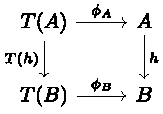
\includegraphics[width=78.0pt]{graphic-02.pdf}  (alg-hom)   
For any endo-functor $T$, $T$-algebras together with $T$-algebra morphisms form a category $\mathcal{A}lg(T)$. We write $\mathcal{U}_{\mathcal{A}lg(T)}:\mathcal{A}lg(T)\to\mathcal{C}$ for the forgetful functor of $\mathcal{A}lg(T)$.\par
 
% END A4.SS4.p1
  
% BEGIN Thmtheorem43
 
\par\medskip\noindent\textbf{Theorem 43 ().}\par
 
% BEGIN Thmtheorem43.p1
 
Let $T$ be an endo-functor on $\mathcal{C}$. The category $\mathcal{A}lg(T)$ is complete whenever $\mathcal{C}$ is.\par
 
% END Thmtheorem43.p1
 
% END Thmtheorem43
 
% BEGIN A4.SS4.SSS0.P0.SPx1
 
\par\medskip\noindent\textbf{Proof.}\par
 
% BEGIN A4.SS4.SSS0.P0.SPx1.p1
 
Let $F:\mathcal{J}\to\mathcal{A}lg(T)$ be a diagram of $T$-algebras. We endow the limit of the $\mathcal{C}$ diagram $\mathcal{U}_{\mathcal{A}lg(T)}\circ F$ with an algebra structure. Let $L$ be the limit of this diagram with projections $\Pi^{L}_{J}:L\to F(J)$. The morphisms $\phi_{F(J)}\circ T(\Pi^{L}_{J}):T(L)\to F(J)$ form a cone on the diagram $\mathcal{U}_{\mathcal{A}lg(T)}\circ F$. We define $\phi_{L}:T(L)\to L$ as the unique morphism into the limit $L$ from this cone. That is,\par
 
\begin{center}\resizebox{\linewidth}{!}{$\begin{aligned}\displaystyle\phi_{L}:=\lim_{J\in\mathcal{J}}\left(\phi_{F(J)}\circ T(\Pi^{L}_{J})\right)\end{aligned}$}\end{center}
 
It remains to show that the projections of the limit $\Pi^{L}_{J}:L\to F(J)$ are algebra homomorphisms, and that given any cone over $F$ in the category $\mathcal{A}lg(T)$ there is a unique $T$-algebra homomorphism from that cone to $(L,\phi_{L})$. We leave the latter as a simple exercise. As for the former, we need to show that the following diagram commutes\par
    
\begin{center}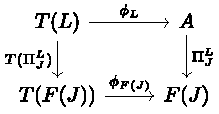
\includegraphics[width=0.95\linewidth,height=0.45\textheight,keepaspectratio]{graphic-03.pdf}\end{center}
    
which simply holds by the definition of $\phi_{L}$ above. $\hfill\blacktriangleleft$\par
 
% END A4.SS4.SSS0.P0.SPx1.p1
 
% BEGIN Thmtheorem44
 
\par\medskip\noindent\textbf{$\blacktriangleright$ Remark 44 ().}\par
 
% BEGIN Thmtheorem44.p1
 
For any $T$-algebra $(A,\phi_{A})$, $(T(A),T(\phi_{A}))$ is also a $T$-algebra. Furthermore, if $h$ is a $T$-algebra morphism, so is $T(h)$. Thus, $T$ forms an endo-functor on the category of $T$-algebras. Consequently, the image of any commutative diagram in $\mathcal{A}lg(T)$ under $T$ is also a commutative diagram. Hence, for a diagram $F:\mathcal{J}\to\mathcal{A}lg(T)$ of $T$-algebras and a cone $\left((A,\phi_{A}),\left\{S_{j}:A\to F(J)\right\}_{j\in J}\right)$ on diagram $F$, the cone below is also a cone on diagram $F$:\par
    \[\left((T(A),T(\phi_{A})),\left\{\phi_{F(J)}\circ T(S_{J}):T(A)\to F(J)\right\}_{j\in J}\right)\]    
% END Thmtheorem44.p1
 
% END Thmtheorem44
 
% BEGIN A4.SS4.SSS0.P0.SPx1.p2
 
\par
 
% END A4.SS4.SSS0.P0.SPx1.p2
 
% END A4.SS4.SSS0.P0.SPx1
 
% END A4.SS4
 
% END A4

\begin{thebibliography}{99}
\bibitem{bib-bib1} 
\par\noindent    Amal Ahmed, Derek Dreyer, and Andreas Rossberg.  State-dependent representation independence.  In Zhong Shao and Benjamin C. Pierce, editors, Proceedings of the 36th ACM SIGPLAN-SIGACT Symposium on Principles of Programming Languages, POPL 2009, Savannah, GA, USA, January 21-23, 2009, pages 340–353. ACM, 2009.  doi:10.1145/1480881.1480925.  

\bibitem{bib-bib2} 
\par\noindent    Benedikt Ahrens, Krzysztof Kapulkin, and Michael Shulman.  Univalent categories and the Rezk completion.  Math. Struct. Comput. Sci., 25(5):1010–1039, 2015.  doi:10.1017/S0960129514000486.  

\bibitem{bib-bib3} 
\par\noindent    Pierre America and Jan J. M. M. Rutten.  Solving Reflexive Domain Equations in a Category of Complete Metric Spaces.  J. Comput. Syst. Sci., 39(3):343–375, 1989.  doi:10.1016/0022-0000(89)90027-5.  

\bibitem{bib-bib4} 
\par\noindent    Andrew W. Appel and David A. McAllester.  An indexed model of recursive types for foundational proof-carrying code.  ACM Trans. Program. Lang. Syst., 23(5):657–683, 2001.  doi:10.1145/504709.504712.  

\bibitem{bib-bib5} 
\par\noindent    Steve Awodey.  Category Theory.  Oxford Logic Guides. Oxford University Press, London, England, 2 edition, June 2010.  

\bibitem{bib-bib6} 
\par\noindent    Nick Benton, Andrew Kennedy, and Carsten Varming.  Some Domain Theory and Denotational Semantics in Coq.  In Stefan Berghofer, Tobias Nipkow, Christian Urban, and Makarius Wenzel, editors, Theorem Proving in Higher Order Logics, 22nd International Conference, TPHOLs 2009, Munich, Germany, August 17-20, 2009. Proceedings, volume 5674 of Lecture Notes in Computer Science, pages 115–130. Springer, 2009.  doi:10.1007/978-3-642-03359-9\_10.  

\bibitem{bib-bib7} 
\par\noindent    Lars Birkedal, Ales Bizjak, and Jan Schwinghammer.  Step-Indexed Relational Reasoning for Countable Nondeterminism.  Log. Methods Comput. Sci., 9(4), 2013.  doi:10.2168/LMCS-9(4:4)2013.  

\bibitem{bib-bib8} 
\par\noindent    Lars Birkedal and Aleš Bizjak.  Lecture Notes on Iris: Higher-Order Concurrent Separation Logic, 2017.  URL: http://iris-project.org/tutorial-pdfs/iris-lecture-notes.pdf.  

\bibitem{bib-bib9} 
\par\noindent    Lars Birkedal, Rasmus Ejlers Møgelberg, Jan Schwinghammer, and Kristian Støvring.  First steps in synthetic guarded domain theory: step-indexing in the topos of trees.  Log. Methods Comput. Sci., 8(4), 2012.  doi:10.2168/LMCS-8(4:1)2012.  

\bibitem{bib-bib10} 
\par\noindent    Lars Birkedal, Bernhard Reus, Jan Schwinghammer, Kristian Støvring, Jacob Thamsborg, and Hongseok Yang.  Step-indexed kripke models over recursive worlds.  In Thomas Ball and Mooly Sagiv, editors, Proceedings of the 38th ACM SIGPLAN-SIGACT Symposium on Principles of Programming Languages, POPL 2011, Austin, TX, USA, January 26-28, 2011, pages 119–132. ACM, 2011.  doi:10.1145/1926385.1926401.  

\bibitem{bib-bib11} 
\par\noindent    Lars Birkedal, Kristian Støvring, and Jacob Thamsborg.  The category-theoretic solution of recursive metric-space equations.  Theor. Comput. Sci., 411(47):4102–4122, 2010.  doi:10.1016/J.TCS.2010.07.010.  

\bibitem{bib-bib12} 
\par\noindent    Errett Bishop.  Foundations of Constructive Analysis.  Mcgraw-Hill, New York, NY, USA, 1967.  

\bibitem{bib-bib13} 
\par\noindent    Ales Bizjak, Lars Birkedal, and Marino Miculan.  A Model of Countable Nondeterminism in Guarded Type Theory.  In Gilles Dowek, editor, Rewriting and Typed Lambda Calculi - Joint International Conference, RTA-TLCA 2014, Held as Part of the Vienna Summer of Logic, VSL 2014, Vienna, Austria, July 14-17, 2014. Proceedings, volume 8560 of Lecture Notes in Computer Science, pages 108–123. Springer, 2014.  doi:10.1007/978-3-319-08918-8\_8.  

\bibitem{bib-bib14} 
\par\noindent    Ranald Clouston, Ales Bizjak, Hans Bugge Grathwohl, and Lars Birkedal.  Programming and Reasoning with Guarded Recursion for Coinductive Types.  In Andrew M. Pitts, editor, Foundations of Software Science and Computation Structures - 18th International Conference, FoSSaCS 2015, Held as Part of the European Joint Conferences on Theory and Practice of Software, ETAPS 2015, London, UK, April 11-18, 2015. Proceedings, volume 9034 of Lecture Notes in Computer Science, pages 407–421. Springer, 2015.  doi:10.1007/978-3-662-46678-0\_26.  

\bibitem{bib-bib15} 
\par\noindent    Robert Dockins.  Formalized, Effective Domain Theory in Coq.  In Gerwin Klein and Ruben Gamboa, editors, Interactive Theorem Proving - 5th International Conference, ITP 2014, Held as Part of the Vienna Summer of Logic, VSL 2014, Vienna, Austria, July 14-17, 2014. Proceedings, volume 8558 of Lecture Notes in Computer Science, pages 209–225. Springer, 2014.  doi:10.1007/978-3-319-08970-6\_14.  

\bibitem{bib-bib16} 
\par\noindent    Peter Freyd.  Algebraically complete categories.  In Aurelio Carboni, Maria Cristina Pedicchio, and Guiseppe Rosolini, editors, Category Theory, pages 95–104, Berlin, Heidelberg, 1991. Springer Berlin Heidelberg.  

\bibitem{bib-bib17} 
\par\noindent    Dan Frumin, Amin Timany, and Lars Birkedal.  Modular Denotational Semantics for Effects with Guarded Interaction Trees.  Proc. ACM Program. Lang., 8(POPL):332–361, 2024.  doi:10.1145/3632854.  

\bibitem{bib-bib18} 
\par\noindent    Pietro Di Gianantonio and Marino Miculan.  A unifying approach to recursive and co-recursive definitions.  In Herman Geuvers and Freek Wiedijk, editors, Types for Proofs and Programs, Second International Workshop, TYPES 2002, Berg en Dal, The Netherlands, April 24-28, 2002, Selected Papers, volume 2646 of Lecture Notes in Computer Science, pages 148–161. Springer, 2002.  doi:10.1007/3-540-39185-1\_9.  

\bibitem{bib-bib19} 
\par\noindent    Pietro Di Gianantonio and Marino Miculan.  Unifying recursive and co-recursive definitions in sheaf categories.  In Igor Walukiewicz, editor, Foundations of Software Science and Computation Structures, 7th International Conference, FOSSACS 2004, Held as Part of the Joint European Conferences on Theory and Practice of Software, ETAPS 2004, Barcelona, Spain, March 29 - April 2, 2004, Proceedings, volume 2987 of Lecture Notes in Computer Science, pages 136–150. Springer, 2004.  doi:10.1007/978-3-540-24727-2\_11.  

\bibitem{bib-bib20} 
\par\noindent    Gaëtan Gilbert, Jesper Cockx, Matthieu Sozeau, and Nicolas Tabareau.  Definitional proof-irrelevance without K.  Proc. ACM Program. Lang., 3(POPL):3:1–3:28, 2019.  doi:10.1145/3290316.  

\bibitem{bib-bib21} 
\par\noindent    Jason Gross, Adam Chlipala, and David I. Spivak.  Experience Implementing a Performant Category-Theory Library in Coq.  In Gerwin Klein and Ruben Gamboa, editors, Interactive Theorem Proving - 5th International Conference, ITP 2014, Held as Part of the Vienna Summer of Logic, VSL 2014, Vienna, Austria, July 14-17, 2014. Proceedings, volume 8558 of Lecture Notes in Computer Science, pages 275–291. Springer, 2014.  doi:10.1007/978-3-319-08970-6\_18.  

\bibitem{bib-bib22} 
\par\noindent    Carl A. Gunter.  Universal Profinite Domains.  Inf. Comput., 72(1):1–30, 1987.  doi:10.1016/0890-5401(87)90048-4.  

\bibitem{bib-bib23} 
\par\noindent    Michael Hedberg.  A coherence theorem for martin-löf’s type theory.  J. Funct. Program., 8(4):413–436, 1998.  doi:10.1017/S0956796898003153.  

\bibitem{bib-bib24} 
\par\noindent    Jason Z. S. Hu and Jacques Carette.  Formalizing category theory in Agda.  In Catalin Hritcu and Andrei Popescu, editors, CPP ’21: 10th ACM SIGPLAN International Conference on Certified Programs and Proofs, Virtual Event, Denmark, January 17-19, 2021, pages 327–342. ACM, 2021.  doi:10.1145/3437992.3439922.  

\bibitem{bib-bib25} 
\par\noindent    Gérard P. Huet and Amokrane Saïbi.  Constructive category theory.  In Gordon D. Plotkin, Colin Stirling, and Mads Tofte, editors, Proof, Language, and Interaction, Essays in Honour of Robin Milner, pages 239–276. The MIT Press, 2000.  

\bibitem{bib-bib26} 
\par\noindent    Brian Huffman.  A Purely Definitional Universal Domain.  In Stefan Berghofer, Tobias Nipkow, Christian Urban, and Makarius Wenzel, editors, Theorem Proving in Higher Order Logics, 22nd International Conference, TPHOLs 2009, Munich, Germany, August 17-20, 2009. Proceedings, volume 5674 of Lecture Notes in Computer Science, pages 260–275. Springer, 2009.  doi:10.1007/978-3-642-03359-9\_19.  

\bibitem{bib-bib27} 
\par\noindent    Thomas Jech.  Set Theory.  Springer Berlin Heidelberg, 2003.  doi:10.1007/3-540-44761-x.  

\bibitem{bib-bib28} 
\par\noindent    Ralf Jung, Robbert Krebbers, Lars Birkedal, and Derek Dreyer.  Higher-order ghost state.  In Jacques Garrigue, Gabriele Keller, and Eijiro Sumii, editors, Proceedings of the 21st ACM SIGPLAN International Conference on Functional Programming, ICFP 2016, Nara, Japan, September 18-22, 2016, pages 256–269. ACM, 2016.  doi:10.1145/2951913.2951943.  

\bibitem{bib-bib29} 
\par\noindent    Ralf Jung, Robbert Krebbers, Jacques-Henri Jourdan, Ales Bizjak, Lars Birkedal, and Derek Dreyer.  Iris from the ground up: A modular foundation for higher-order concurrent separation logic.  J. Funct. Program., 28:e20, 2018.  doi:10.1017/S0956796818000151.  

\bibitem{bib-bib30} 
\par\noindent    Max Kelly.  Basic concepts of enriched category theory series number 64.  London Mathematical Society lecture note series. Cambridge University Press, Cambridge, England, February 1982.  

\bibitem{bib-bib31} 
\par\noindent    Dominik Kirst and Gert Smolka.  Large model constructions for second-order ZF in dependent type theory.  In June Andronick and Amy P. Felty, editors, Proceedings of the 7th ACM SIGPLAN International Conference on Certified Programs and Proofs, CPP 2018, Los Angeles, CA, USA, January 8-9, 2018, pages 228–239. ACM, 2018.  doi:10.1145/3167095.  

\bibitem{bib-bib32} 
\par\noindent    Robbert Krebbers, Jacques-Henri Jourdan, Ralf Jung, Joseph Tassarotti, Jan-Oliver Kaiser, Amin Timany, Arthur Charguéraud, and Derek Dreyer.  Mosel: a general, extensible modal framework for interactive proofs in separation logic.  Proc. ACM Program. Lang., 2(ICFP):77:1–77:30, 2018.  doi:10.1145/3236772.  

\bibitem{bib-bib33} 
\par\noindent    Robbert Krebbers, Amin Timany, and Lars Birkedal.  Interactive proofs in higher-order concurrent separation logic.  In Giuseppe Castagna and Andrew D. Gordon, editors, Proceedings of the 44th ACM SIGPLAN Symposium on Principles of Programming Languages, POPL 2017, Paris, France, January 18-20, 2017, pages 205–217. ACM, 2017.  doi:10.1145/3009837.3009855.  

\bibitem{bib-bib34} 
\par\noindent    Saunders Mac Lane.  Categories for the working mathematician.  Graduate Texts in Mathematics. Springer, New York, NY, 2 edition, September 1998.  

\bibitem{bib-bib35} 
\par\noindent    Saunders MacLane and Ieke Moerdijk.  Sheaves in geometry and logic.  Universitext. Springer, New York, NY, 1 edition, May 1992.  

\bibitem{bib-bib36} 
\par\noindent    The mathlib Community.  The lean mathematical library.  In Proceedings of the 9th ACM SIGPLAN International Conference on Certified Programs and Proofs, CPP 2020, pages 367–381, New York, NY, USA, 2020. Association for Computing Machinery.  doi:10.1145/3372885.3373824.  

\bibitem{bib-bib37} 
\par\noindent    Hiroshi Nakano.  A Modality for Recursion.  In 15th Annual IEEE Symposium on Logic in Computer Science, Santa Barbara, California, USA, June 26-29, 2000, pages 255–266. IEEE Computer Society, 2000.  doi:10.1109/LICS.2000.855774.  

\bibitem{bib-bib38} 
\par\noindent    Christine Paulin-Mohring.  A constructive denotational semantics for Kahn networks in Coq.  In Yves Bertot, Gérard Huet, Jean-Jacques Lévy, and Gordon Plotkin, editors, From Semantics to Computer Science, pages 383–413. Cambridge University Press, 2009.  URL: https://inria.hal.science/inria-00431806.  

\bibitem{bib-bib39} 
\par\noindent    Marco Paviotti, Rasmus Ejlers Møgelberg, and Lars Birkedal.  A model of PCF in guarded type theory.  In Dan R. Ghica, editor, The 31st Conference on the Mathematical Foundations of Programming Semantics, MFPS 2015, Nijmegen, The Netherlands, June 22-25, 2015, volume 319 of Electronic Notes in Theoretical Computer Science, pages 333–349. Elsevier, 2015.  doi:10.1016/J.ENTCS.2015.12.020.  

\bibitem{bib-bib40} 
\par\noindent    Daniel Peebles, James Deikun, Ulf Norell, Dan Doel, Darius Jahandarie, and James Cook.  categories: Categories parametrized by morphism equality in Agda.  https://github.com/copumpkin/categories, 2018.  

\bibitem{bib-bib41} 
\par\noindent    Dana Scott.  Outline of a mathematical theory of computation.  Technical Report PRG02, OUCL, November 1970.  

\bibitem{bib-bib42} 
\par\noindent    Dana Scott.  Continuous lattices.  In F. W. Lawvere, editor, Toposes, Algebraic Geometry and Logic, pages 97–136, Berlin, Heidelberg, 1972. Springer Berlin Heidelberg.  

\bibitem{bib-bib43} 
\par\noindent    Filip Sieczkowski, Ales Bizjak, and Lars Birkedal.  ModuRes: A Coq Library for Modular Reasoning About Concurrent Higher-Order Imperative Programming Languages.  In Christian Urban and Xingyuan Zhang, editors, Interactive Theorem Proving - 6th International Conference, ITP 2015, Nanjing, China, August 24-27, 2015, Proceedings, volume 9236 of Lecture Notes in Computer Science, pages 375–390. Springer, 2015.  doi:10.1007/978-3-319-22102-1\_25.  

\bibitem{bib-bib44} 
\par\noindent    Michael B. Smyth and Gordon D. Plotkin.  The Category-Theoretic Solution of Recursive Domain Equations.  SIAM J. Comput., 11(4):761–783, 1982.  doi:10.1137/0211062.  

\bibitem{bib-bib45} 
\par\noindent    Simon Spies, Lennard Gäher, Daniel Gratzer, Joseph Tassarotti, Robbert Krebbers, Derek Dreyer, and Lars Birkedal.  Transfinite Iris: resolving an existential dilemma of step-indexed separation logic.  In Stephen N. Freund and Eran Yahav, editors, PLDI ’21: 42nd ACM SIGPLAN International Conference on Programming Language Design and Implementation, Virtual Event, Canada, June 20-25, 2021, pages 80–95. ACM, 2021.  doi:10.1145/3453483.3454031.  

\bibitem{bib-bib46} 
\par\noindent    Sergei Stepanenko and Amin Timany.  The Rocq Mechanization of Solving Guarded Domain Equations in Presheaves Over Ordinals.  https://doi.org/10.5281/zenodo.15406039.  

\bibitem{bib-bib47} 
\par\noindent    V. Stoltenberg-Hansen, I. Lindström, and E. R. Griffor.  Mathematical Theory of Domains.  Cambridge Tracts in Theoretical Computer Science. Cambridge University Press, 1994.  

\bibitem{bib-bib48} 
\par\noindent    Amin Timany.  Commuting Quantifiers, October 2020.  Blog post, accessed on Feb 8, 2025.  URL: https://cs.au.dk/˜timany/blog/commuting\_quantifiers/.  

\bibitem{bib-bib49} 
\par\noindent    Amin Timany and Bart Jacobs.  Category Theory in Coq 8.5.  In Delia Kesner and Brigitte Pientka, editors, 1st International Conference on Formal Structures for Computation and Deduction (FSCD 2016), volume 52 of Leibniz International Proceedings in Informatics (LIPIcs), pages 30:1–30:18, Dagstuhl, Germany, 2016. Schloss Dagstuhl – Leibniz-Zentrum für Informatik.  doi:10.4230/LIPIcs.FSCD.2016.30.  

\bibitem{bib-bib50} 
\par\noindent    The Univalent Foundations Program.  Homotopy Type Theory: Univalent Foundations of Mathematics.  https://homotopytypetheory.org/book, Institute for Advanced Study, 2013.  

\bibitem{bib-bib51} 
\par\noindent    Mitchell Wand.  Fixed-Point Constructions in Order-Enriched Categories.  Theor. Comput. Sci., 8:13–30, 1979.  doi:10.1016/0304-3975(79)90053-7.  

\bibitem{bib-bib52} 
\par\noindent    John Wiegley.  category-theory: Category Theory in Coq.  https://github.com/jwiegley/category-theory, 2019.  

\end{thebibliography}
\end{document}
